\documentclass{beamer}

\newcommand{\collegeBeamerRoot}{.}
\makeatletter
\def\input@path{{./}}
\makeatother
\usepackage[en,cqu]{collegeBeamer}

\newcommand{\PresenterName}{Xuhang Ye}
\newcommand{\PresenterSchool}{JingLab, Chongqing University}
\newcommand{\PresentationTopic}{Robot Learning and Control\\Group Meeting Report}
\newcommand{\PresentationSubtitle}{Thesis Progress and Research Plan}

\title[Robot Learning and Control]{\PresentationTopic}
\subtitle{\PresentationSubtitle}
\author{\PresenterName \quad \PresenterSchool}
\date{July 11, 2026}

\begin{document}

\maketitle

\begin{frame}{Outline}
    \tableofcontents
\end{frame}

\section{Brief Self-Introduction}

\begin{frame}{Brief Self-Introduction}
    \small
    \setlength{\parskip}{0.55em}

    \textbf{\textcolor{maincolor}{Background:}} B.Eng. in Computer Science and Technology, College of Computer Science, Chongqing University

    \textbf{\textcolor{maincolor}{Relevant Coursework:}} Advanced Mathematics, Linear Algebra, Probability and Statistics, Data Structures and Algorithms, Operating Systems, Machine Learning

    \textbf{\textcolor{maincolor}{Computational Strengths:}} Programming, algorithmic thinking, Linux-based development, machine learning practice, and end-to-end engineering implementation

    \textbf{\textcolor{maincolor}{Research Interest:}} Robot learning, dexterous manipulation, and sim-to-real transfer

    \textbf{\textcolor{maincolor}{Links:}} GitHub: \bhref{https://github.com/CQULeaf}{github.com/CQULeaf} \quad Website: \bhref{https://yexuhang.com/}{yexuhang.com}
\end{frame}

\section{Technical Pilot}

\begin{frame}{Pilot Scope and Thesis Link}
    \small
    \begin{columns}[T,onlytextwidth]
        \begin{column}{0.48\textwidth}
            \textbf{\textcolor{maincolor}{Purpose}}
            \begin{itemize}
                \item Learn the LEAP Hand robot-learning stack.
                \item Run a complete loop: modeling, training, playback, and ROS2 hardware deployment.
                \item Use the pilot to prepare for the thesis project, not to solve the same task.
            \end{itemize}
        \end{column}
        \begin{column}{0.48\textwidth}
            \textbf{\textcolor{maincolor}{Relation to Thesis}}
            \begin{itemize}
                \item Pilot: cube reorientation around the $z$ axis.
                \item Thesis: continuous cylinder in-hand rotation.
                \item Shared pipeline: proprioception-only policy, relative joint targets, sim-to-real alignment.
            \end{itemize}
        \end{column}
    \end{columns}

    \vspace{0.4em}
    \centering
    \textcolor{maincolor}{Pilot task $\neq$ thesis task; pilot pipeline $\rightarrow$ thesis implementation baseline.}
\end{frame}

\begin{frame}{Task Modeling: From Goal to POMDP}
    \small
    \vspace{0.8em}
    \begin{columns}[T,onlytextwidth]
        \begin{column}{0.48\textwidth}
            \textbf{\textcolor{maincolor}{Manipulation Goal}}
            \begin{itemize}
                \item Hold a cube inside the LEAP Hand.
                \item Track a sequence of local yaw goals.
                \item Reset or terminate when the cube leaves the hand or flips.
            \end{itemize}

            \vspace{0.2em}
            \[
                \mathcal{M}
                =
                \langle
                \mathcal{S},\mathcal{A},\mathcal{O},P,r,\gamma
                \rangle
            \]

            \scriptsize
            $\mathcal{S}$ includes hand state, object pose, contact, and randomized dynamics;
            $\mathcal{O}$ is the deployable proprioceptive observation.
        \end{column}
        \begin{column}{0.48\textwidth}
            \textbf{\textcolor{maincolor}{Goal Update}}
            \[
                q^g_{k+1}
                =
                q_z\!\left(\frac{2\pi}{16}\right)
                \otimes q^g_k
            \]

            \[
                d_R(q^o_t,q^g_t)
                =
                2\arcsin
                \left\|
                \operatorname{vec}(q^o_t \otimes (q^g_t)^{-1})
                \right\|_2
            \]

            \[
                \mathrm{success}
                =
                [d_R \le 0.2]\wedge
                [\|p^o_t-p_{\mathrm{hand}}\|_2 \le 0.025]
            \]

            \[
                \mathrm{done}
                =
                [\|p^o_t-p_{\mathrm{hand}}\|_2 \ge 0.07]\vee
                [\mathrm{timeout}]
            \]
        \end{column}
    \end{columns}
\end{frame}

\begin{frame}{Observation, Action, and Reward}
    \footnotesize
    \vspace{0.7em}
    \begin{columns}[T,onlytextwidth]
        \begin{column}{0.48\textwidth}
            \textbf{\textcolor{maincolor}{Policy Interface}}
            \[
                \tilde q_t =
                \frac{2q_t-q_{\max}-q_{\min}}
                     {q_{\max}-q_{\min}}
            \]
            \[
                x_t=[\tilde q_t,u_t]\in\mathbb{R}^{32}
            \]
            \[
                o_t=
                \operatorname{vec}(x_{t-2},x_{t-1},x_t)
                \in\mathbb{R}^{96}
            \]
            \[
                a_t\in[-1,1]^{16}
            \]
            \[
                u_t=
                \operatorname{clip}
                \left(
                    u_{t-1}+\frac{1}{24}a_t,
                    q_{\min},
                    q_{\max}
                \right)
            \]

            \vspace{0.1em}
            \begin{itemize}
                \item No vision input.
                \item No tactile input.
                \item No object state as policy input.
            \end{itemize}
        \end{column}
        \begin{column}{0.48\textwidth}
            \textbf{\textcolor{maincolor}{Reward Design}}
            \[
                r_t =
                w_p\|p^o_t-p_{\mathrm{hand}}\|_2
                +
                \frac{w_R}{d_R+\epsilon}
            \]
            \[
                \quad
                +w_a\|a_t\|_2^2
                +w_q\|u_t-q_{\mathrm{grasp}}\|_2^2
                +b_{\mathrm{success}}
                +b_{\mathrm{fall}}
            \]

            \vspace{0.1em}
            \begin{itemize}
                \item Position term keeps the cube near the hand.
                \item Rotation term tracks the current goal.
                \item Regularizers suppress large or unstable motions.
                \item Bonus/penalty handles success and falling.
            \end{itemize}
        \end{column}
    \end{columns}
\end{frame}

\begin{frame}{Training in Isaac Lab}
    \small
    \centering
    \begin{columns}[T,onlytextwidth]
        \begin{column}{0.23\textwidth}
            \centering
            \textbf{\textcolor{maincolor}{Environment}}\\
            \vspace{0.2em}
            \scriptsize
            Isaac Lab \texttt{DirectRLEnv}\\
            task registration\\
            reset / reward / done
        \end{column}
        \begin{column}{0.23\textwidth}
            \centering
            \textbf{\textcolor{maincolor}{Sampling}}\\
            \vspace{0.2em}
            \scriptsize
            $8192$ parallel envs\\
            $dt=1/120$ s\\
            decimation $=4$
        \end{column}
        \begin{column}{0.23\textwidth}
            \centering
            \textbf{\textcolor{maincolor}{Policy}}\\
            \vspace{0.2em}
            \scriptsize
            \texttt{rl\_games} PPO\\
            MLP $[512,256,128]$\\
            GRU $256$
        \end{column}
        \begin{column}{0.23\textwidth}
            \centering
            \textbf{\textcolor{maincolor}{Checkpoint}}\\
            \vspace{0.2em}
            \scriptsize
            train / resume\\
            sim playback\\
            deployment restore
        \end{column}
    \end{columns}

    \vspace{0.9em}
    \[
        \text{Isaac Lab rollout}
        \rightarrow
        \text{PPO update}
        \rightarrow
        \text{checkpoint}
        \rightarrow
        \text{playback / deployment}
    \]

    \vspace{0.4em}
    \begin{columns}[T,onlytextwidth]
        \begin{column}{0.48\textwidth}
            \textbf{\textcolor{maincolor}{Domain Randomization}}
            \begin{itemize}
                \item friction, mass, stiffness/damping
                \item initial pose noise and object wrench
            \end{itemize}
        \end{column}
        \begin{column}{0.48\textwidth}
            \textbf{\textcolor{maincolor}{Control Robustness}}
            \begin{itemize}
                \item action noise and action latency
                \item no observation latency in this pilot
            \end{itemize}
        \end{column}
    \end{columns}
\end{frame}

\begin{frame}{From Simulation to ROS2 Hardware}
    \small
    \begin{columns}[T,onlytextwidth]
        \begin{column}{0.48\textwidth}
            \href{run:assets/videos/sim_reorientation.mp4}{%
                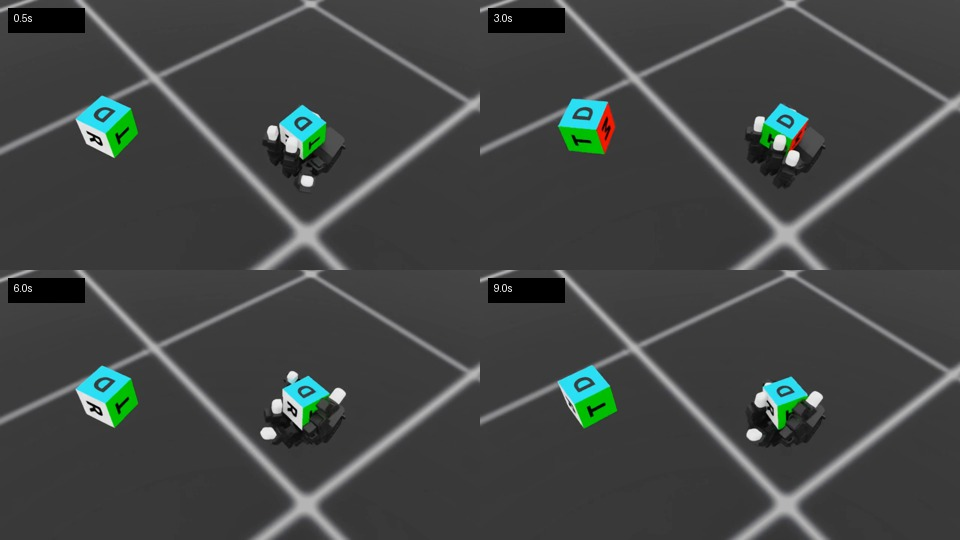
\includegraphics[width=\textwidth]{assets/figures/sim_reorientation_keyframes.jpg}}
            \centering
            \scriptsize Simulation rollout
        \end{column}
        \begin{column}{0.48\textwidth}
            \href{run:assets/videos/real_reorientation_ros2.mp4}{%
                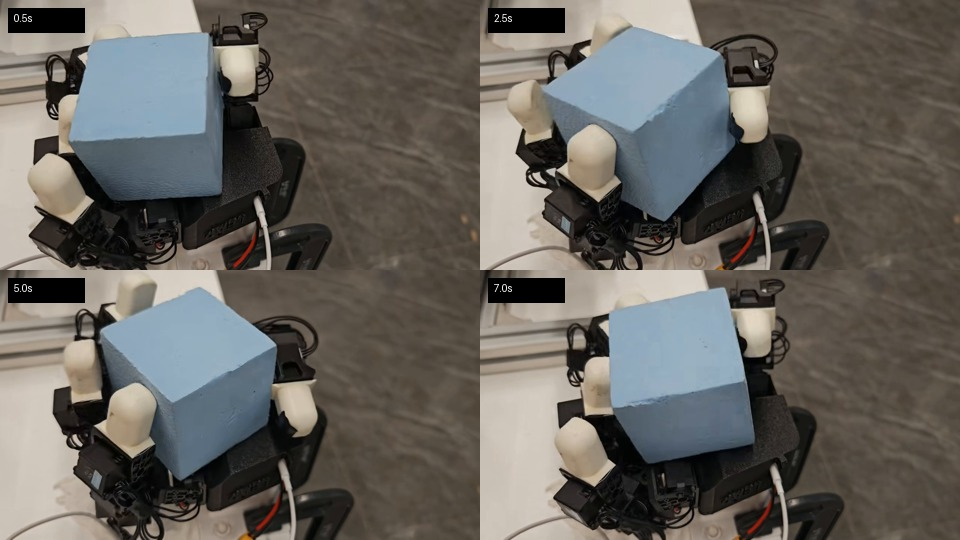
\includegraphics[width=\textwidth]{assets/figures/real_reorientation_keyframes.jpg}}
            \centering
            \scriptsize ROS2 hardware demo
        \end{column}
    \end{columns}

    \vspace{0.5em}
    \begin{columns}[T,onlytextwidth]
        \begin{column}{0.32\textwidth}
            \centering
            \textbf{\textcolor{maincolor}{Checkpoint}}\\
            \scriptsize restore trained policy
        \end{column}
        \begin{column}{0.32\textwidth}
            \centering
            \textbf{\textcolor{maincolor}{Observation}}\\
            \scriptsize same $96$D history
        \end{column}
        \begin{column}{0.32\textwidth}
            \centering
            \textbf{\textcolor{maincolor}{Action}}\\
            \scriptsize same relative target update
        \end{column}
    \end{columns}

    \vspace{0.65em}
    \centering
    \scriptsize Key alignment issues: joint order, normalization, action scale, control rate, and safety limits.
\end{frame}

\section{Thesis Project}

\begin{frame}{Thesis Project: Continuous In-Hand Rotation}
    \small
    \vspace{0.75em}
    \begin{columns}[T,onlytextwidth]
        \begin{column}{0.48\textwidth}
            \textbf{\textcolor{maincolor}{Research Question}}
            \begin{itemize}
                \item Can a low-cost LEAP Hand learn continuous in-hand cylinder rotation?
                \item Can the final policy run without vision, tactile sensing, or real object parameters?
                \item Where does the learned skill fail on real objects?
            \end{itemize}
        \end{column}
        \begin{column}{0.48\textwidth}
            \textbf{\textcolor{maincolor}{From Pilot to Thesis}}
            \begin{itemize}
                \item Pilot: discrete cube reorientation.
                \item Thesis: sustained cylinder rotation.
                \item Shared interface: proprioception and relative joint targets.
            \end{itemize}
        \end{column}
    \end{columns}

    \vspace{0.45em}
    \centering
    \textcolor{maincolor}{Pilot task $\rightarrow$ implementation baseline; thesis task $\rightarrow$ research contribution.}
\end{frame}

\begin{frame}{Task Definition: Sustained Rotation}
    \small
    \vspace{0.7em}
    \begin{columns}[T,onlytextwidth]
        \begin{column}{0.46\textwidth}
            \textbf{\textcolor{maincolor}{Goal}}
            \begin{itemize}
                \item Hold a cylinder inside the hand.
                \item Keep rotating around the vertical axis.
                \item Survive a fixed $20\,\mathrm{s}$ episode.
            \end{itemize}

            \vspace{0.25em}
            \[
                e_z = [0,0,1]^\top
            \]
            \[
                \Delta Q_t
                =
                Q_t^o \otimes (Q_{t-1}^o)^{-1}
            \]
            \[
                \omega_t^{\parallel}
                =
                e_z^\top
                \frac{\operatorname{Log}(\Delta Q_t)}{\Delta t}
            \]
        \end{column}
        \begin{column}{0.50\textwidth}
            \textbf{\textcolor{maincolor}{Key Difference from Reorientation}}
            \begin{itemize}
                \item No fixed terminal orientation.
                \item Reward measures continuous axial spin.
                \item Stability matters as much as rotation speed.
            \end{itemize}

            \vspace{0.35em}
            \[
                \pi^\ast
                =
                \arg\max_\pi
                \mathbb{E}_{\pi}
                \left[
                \sum_{t=0}^{T-1}
                \gamma^t r_t
                \right]
            \]

            \vspace{0.2em}
            \centering
            \textcolor{maincolor}{Reorientation asks ``where to stop''; rotation asks ``how to keep going''.}
        \end{column}
    \end{columns}
\end{frame}

\begin{frame}{Policy Interface: Deployable by Design}
    \footnotesize
    \vspace{0.6em}
    \begin{columns}[T,onlytextwidth]
        \begin{column}{0.48\textwidth}
            \textbf{\textcolor{maincolor}{Observation and Action}}
            \[
                x_t=[\tilde q_t,q_t^{tar}]\in\mathbb{R}^{32}
            \]
            \[
                O_t^\pi=[x_{t-2},x_{t-1},x_t]\in\mathbb{R}^{96}
            \]
            \[
                h_t=[x_{t-29},\ldots,x_t]\in\mathbb{R}^{30\times32}
            \]
            \[
                a_t\in[-1,1]^{16}
            \]
            \[
                q_t^{tar}
                =
                \operatorname{clip}
                \left(q_{t-1}^{tar}+\frac{1}{24}a_t,\ q_{\min},q_{\max}\right)
            \]
        \end{column}
        \begin{column}{0.48\textwidth}
            \textbf{\textcolor{maincolor}{Training-Only Privileged Information}}
            \[
                \xi_t =
                [p_t^o,\rho,m,\mu,c^\top]^\top
                \in\mathbb{R}^{9}
            \]

            \vspace{0.2em}
            \begin{tabular}{p{0.48\textwidth}c}
                \hline
                Signal & Real policy input? \\
                \hline
                joint position & yes \\
                joint target history & yes \\
                object pose & no \\
                mass / friction / CoM & no \\
                vision / tactile & no \\
                \hline
            \end{tabular}

            \vspace{0.45em}
            \centering
            \textcolor{maincolor}{The policy interface is constrained before training starts.}
        \end{column}
    \end{columns}
\end{frame}

\begin{frame}{Reward: Rotate, Stabilize, and Control}
    \footnotesize
    \vspace{0.7em}
    \begin{columns}[T,onlytextwidth]
        \begin{column}{0.50\textwidth}
            \textbf{\textcolor{maincolor}{Rotation Term}}
            \[
                r_t^{rot}
                =
                \lambda_{rot}
                \operatorname{clip}
                \left(
                    \omega_t^{\parallel},
                    r_{\min}, r_{\max}
                \right)
            \]

            \vspace{0.3em}
            \textbf{\textcolor{maincolor}{Total Reward}}
            \[
                r_t =
                r_t^{rot}
                + r_t^{pose}
                + r_t^{lin}
                + r_t^\tau
                + r_t^{work}
                + r_t^a
                + r_t^{center}
            \]

            \[
                \mathrm{done}
                =
                [\|p_t^o-p_{\mathrm{hand}}\|_2\ge0.07]
                \vee[t\ge T]
            \]
        \end{column}
        \begin{column}{0.46\textwidth}
            \textbf{\textcolor{maincolor}{Design Intent}}
            \begin{itemize}
                \item reward axial spin, not arbitrary motion;
                \item keep the cylinder near the in-hand center;
                \item suppress linear velocity and pose drift;
                \item penalize torque, work, and action size;
                \item terminate on falling or timeout.
            \end{itemize}

            \vspace{0.35em}
            \centering
            \textcolor{maincolor}{Reward design separates useful rotation from unstable throwing.}
        \end{column}
    \end{columns}
\end{frame}

\begin{frame}{Skill-Prior-Driven Proprioceptive Rotation}
    \footnotesize
    \vspace{0.2em}
    \begin{columns}[T,onlytextwidth]
        \begin{column}{0.73\textwidth}
            \centering
            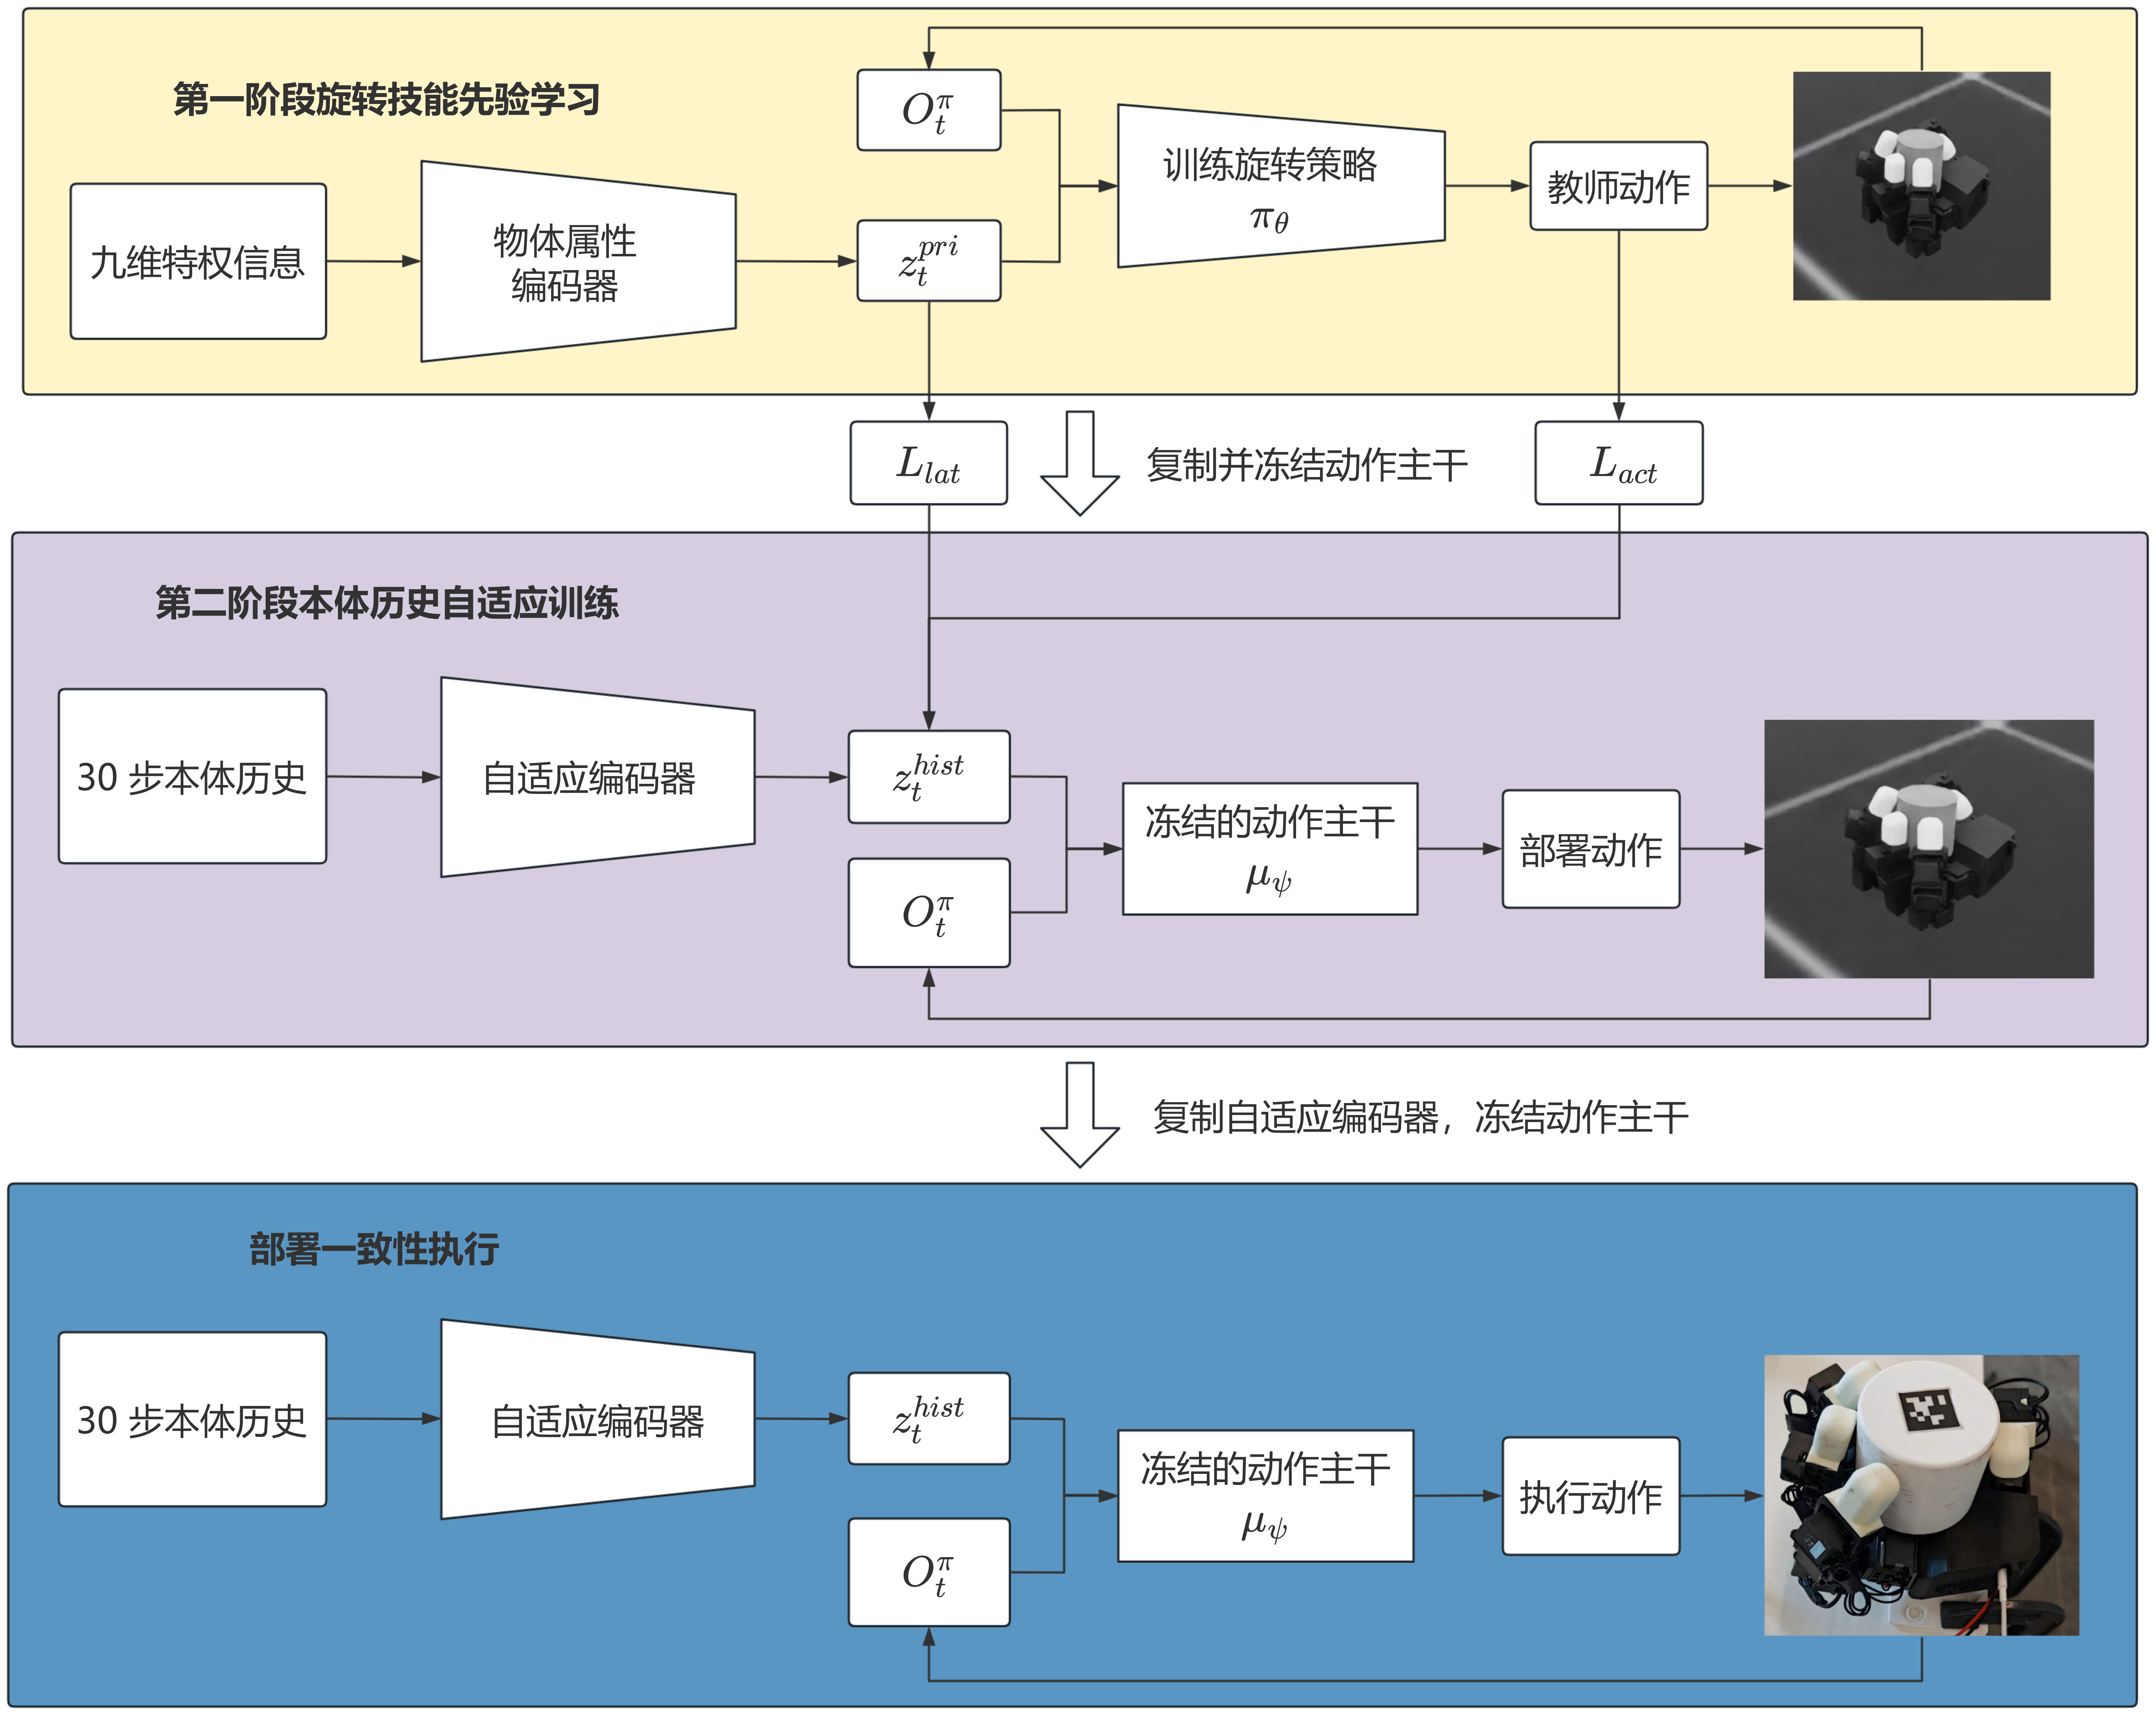
\includegraphics[width=\textwidth,height=0.72\paperheight,keepaspectratio]{assets/figures/rotation/method_framework_cropped.png}
        \end{column}
        \begin{column}{0.23\textwidth}
            \scriptsize
            \vspace{0.9em}
            \textbf{\textcolor{maincolor}{Stage 1}}\\[-0.1em]
            \(z_t^{pri}=E_{pri}(\xi_t)\)\\
            Privileged PPO teacher.

            \vspace{1.15em}
            \textbf{\textcolor{maincolor}{Stage 2}}\\[-0.1em]
            \(z_t^{hist}=E_{hist}(h_t)\)\\
            Train history encoder; freeze actor.

            \vspace{1.15em}
            \textbf{\textcolor{maincolor}{Deployment}}\\[-0.1em]
            \(\mu_t=\mu_\psi([O_t^\pi;z_t^{hist}])\)\\
            No privileged info.

            \vspace{1.25em}
            \textcolor{maincolor}{\rule{0.9\linewidth}{0.4pt}}

            \vspace{0.35em}
            \textbf{\textcolor{maincolor}{Key idea}}\\
            Train with privilege.\\
            Deploy with proprioception.
        \end{column}
    \end{columns}
\end{frame}

\begin{frame}{Training Protocol in Isaac Lab}
    \footnotesize
    \vspace{0.2em}
    \begin{columns}[T,onlytextwidth]
        \begin{column}{0.48\textwidth}
            \textbf{\textcolor{maincolor}{Simulation and Sampling}}

            \vspace{0.15em}
            \resizebox{\textwidth}{!}{%
            \begin{tabular}{ll}
                \hline
                Item & Setting \\
                \hline
                Isaac Lab task & cylinder rotation \\
                Physics / policy rate & $120$ Hz / $30$ Hz \\
                Decimation & $4$ physics steps \\
                Episode length & $20$ s \\
                Action scale & $1/24$ relative target \\
                Evaluation & $128$ episodes per split \\
                \hline
            \end{tabular}
            }

            \vspace{0.45em}
            \textbf{\textcolor{maincolor}{Inputs and Latent}}
            \[
                O_t^\pi \in \mathbb{R}^{96}
                \quad
                h_t \in \mathbb{R}^{30\times32}
                \quad
                z_t \in \mathbb{R}^{8}
            \]
            \scriptsize
            Actor input is short proprioceptive history plus the $8$D skill prior.
        \end{column}
        \begin{column}{0.48\textwidth}
            \textbf{\textcolor{maincolor}{Networks and Optimization}}

            \vspace{0.15em}
            \resizebox{\textwidth}{!}{%
            \begin{tabular}{lll}
                \hline
                Module & Architecture & Used in \\
                \hline
                $E_{pri}$ & MLP $9\!\to\!256\!\to\!128\!\to\!8$ & Teacher \\
                Actor/Critic & MLP $[512,256,128]$ & Stage 1, deploy \\
                $E_{hist}$ & 1D-CNN on $30\times32$ history & Stage 2, deploy \\
                \hline
            \end{tabular}
            }

            \vspace{0.35em}
            \[
                \begin{aligned}
                    z_t^{pri}  &= \tanh(E_{pri}(\xi_t)) \\
                    z_t^{hist} &= \tanh(E_{hist}(h_t))
                \end{aligned}
            \]

            \vspace{-0.25em}
            \begin{itemize}
                \item Stage 1: PPO trains $E_{pri}$ and actor/critic with $8192$ envs.
                \item Stage 2: freeze actor, train $E_{hist}$ with $4096$ envs.
                \item Deploy-Refined: wider CoM range and $\lambda_{act}=1$.
            \end{itemize}

            \vspace{0.15em}
            \centering
            \scriptsize
            Deployment keeps only $E_{hist}$ and the frozen actor.
        \end{column}
    \end{columns}
\end{frame}

\begin{frame}{Training Evidence: Successful Rotation}
    \footnotesize
    \vspace{0.15em}
    \begin{columns}[T,onlytextwidth]
        \begin{column}{0.49\textwidth}
            \centering
            \textbf{\textcolor{maincolor}{Teacher Training}}\\[0.05em]
            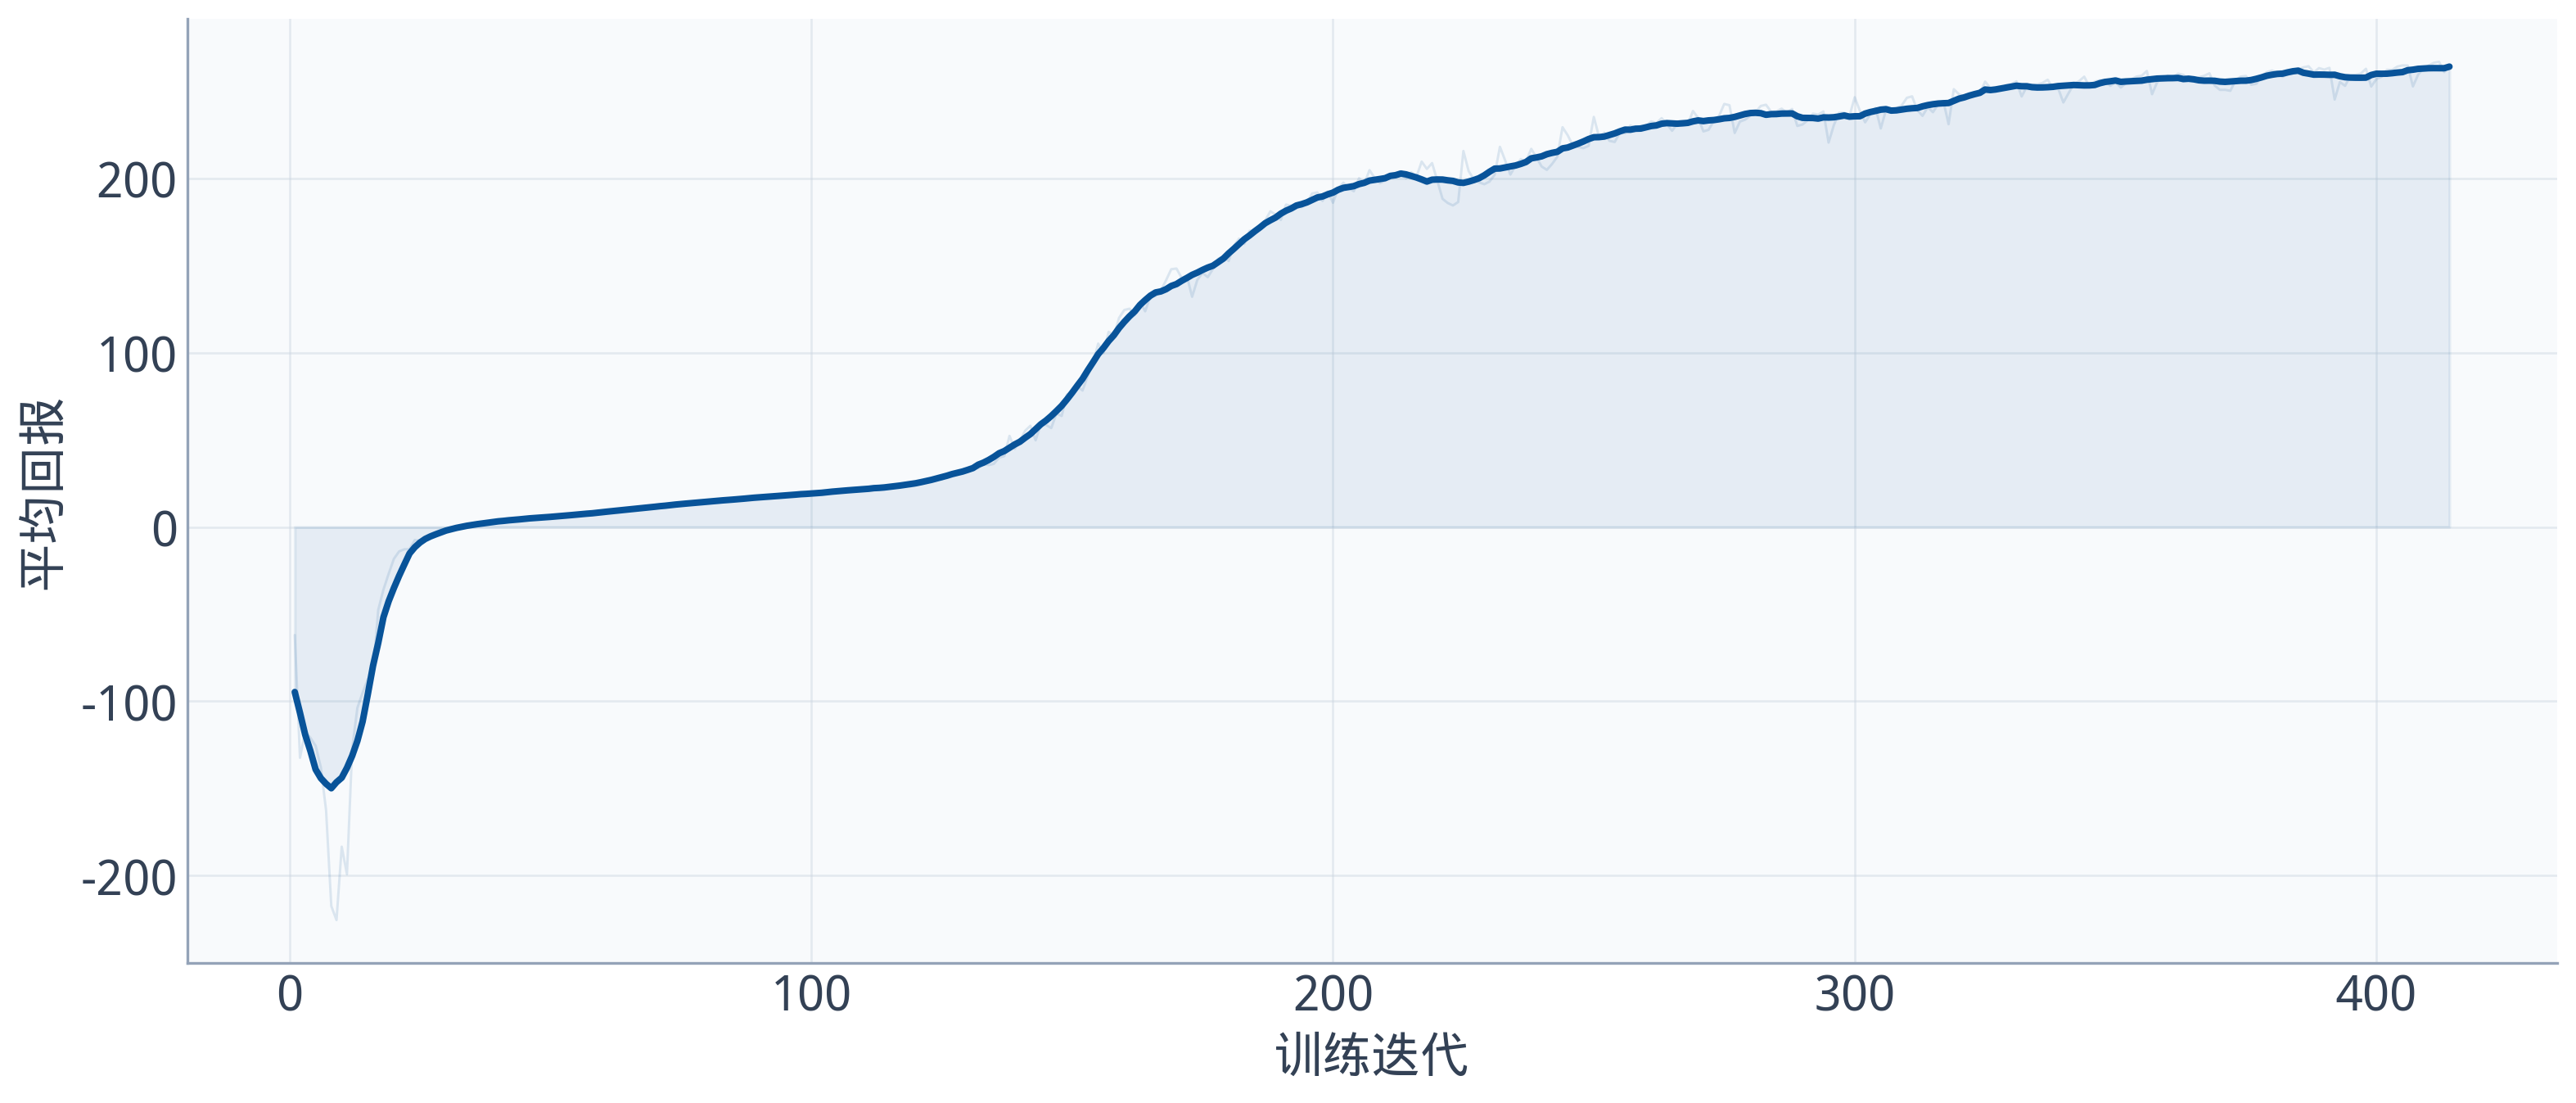
\includegraphics[width=1.22\textwidth,height=0.33\textheight,keepaspectratio]{assets/figures/rotation/stage1_reward_curve.png}
        \end{column}
        \begin{column}{0.49\textwidth}
            \centering
            \textbf{\textcolor{maincolor}{Deploy-Base Training}}\\[0.05em]
            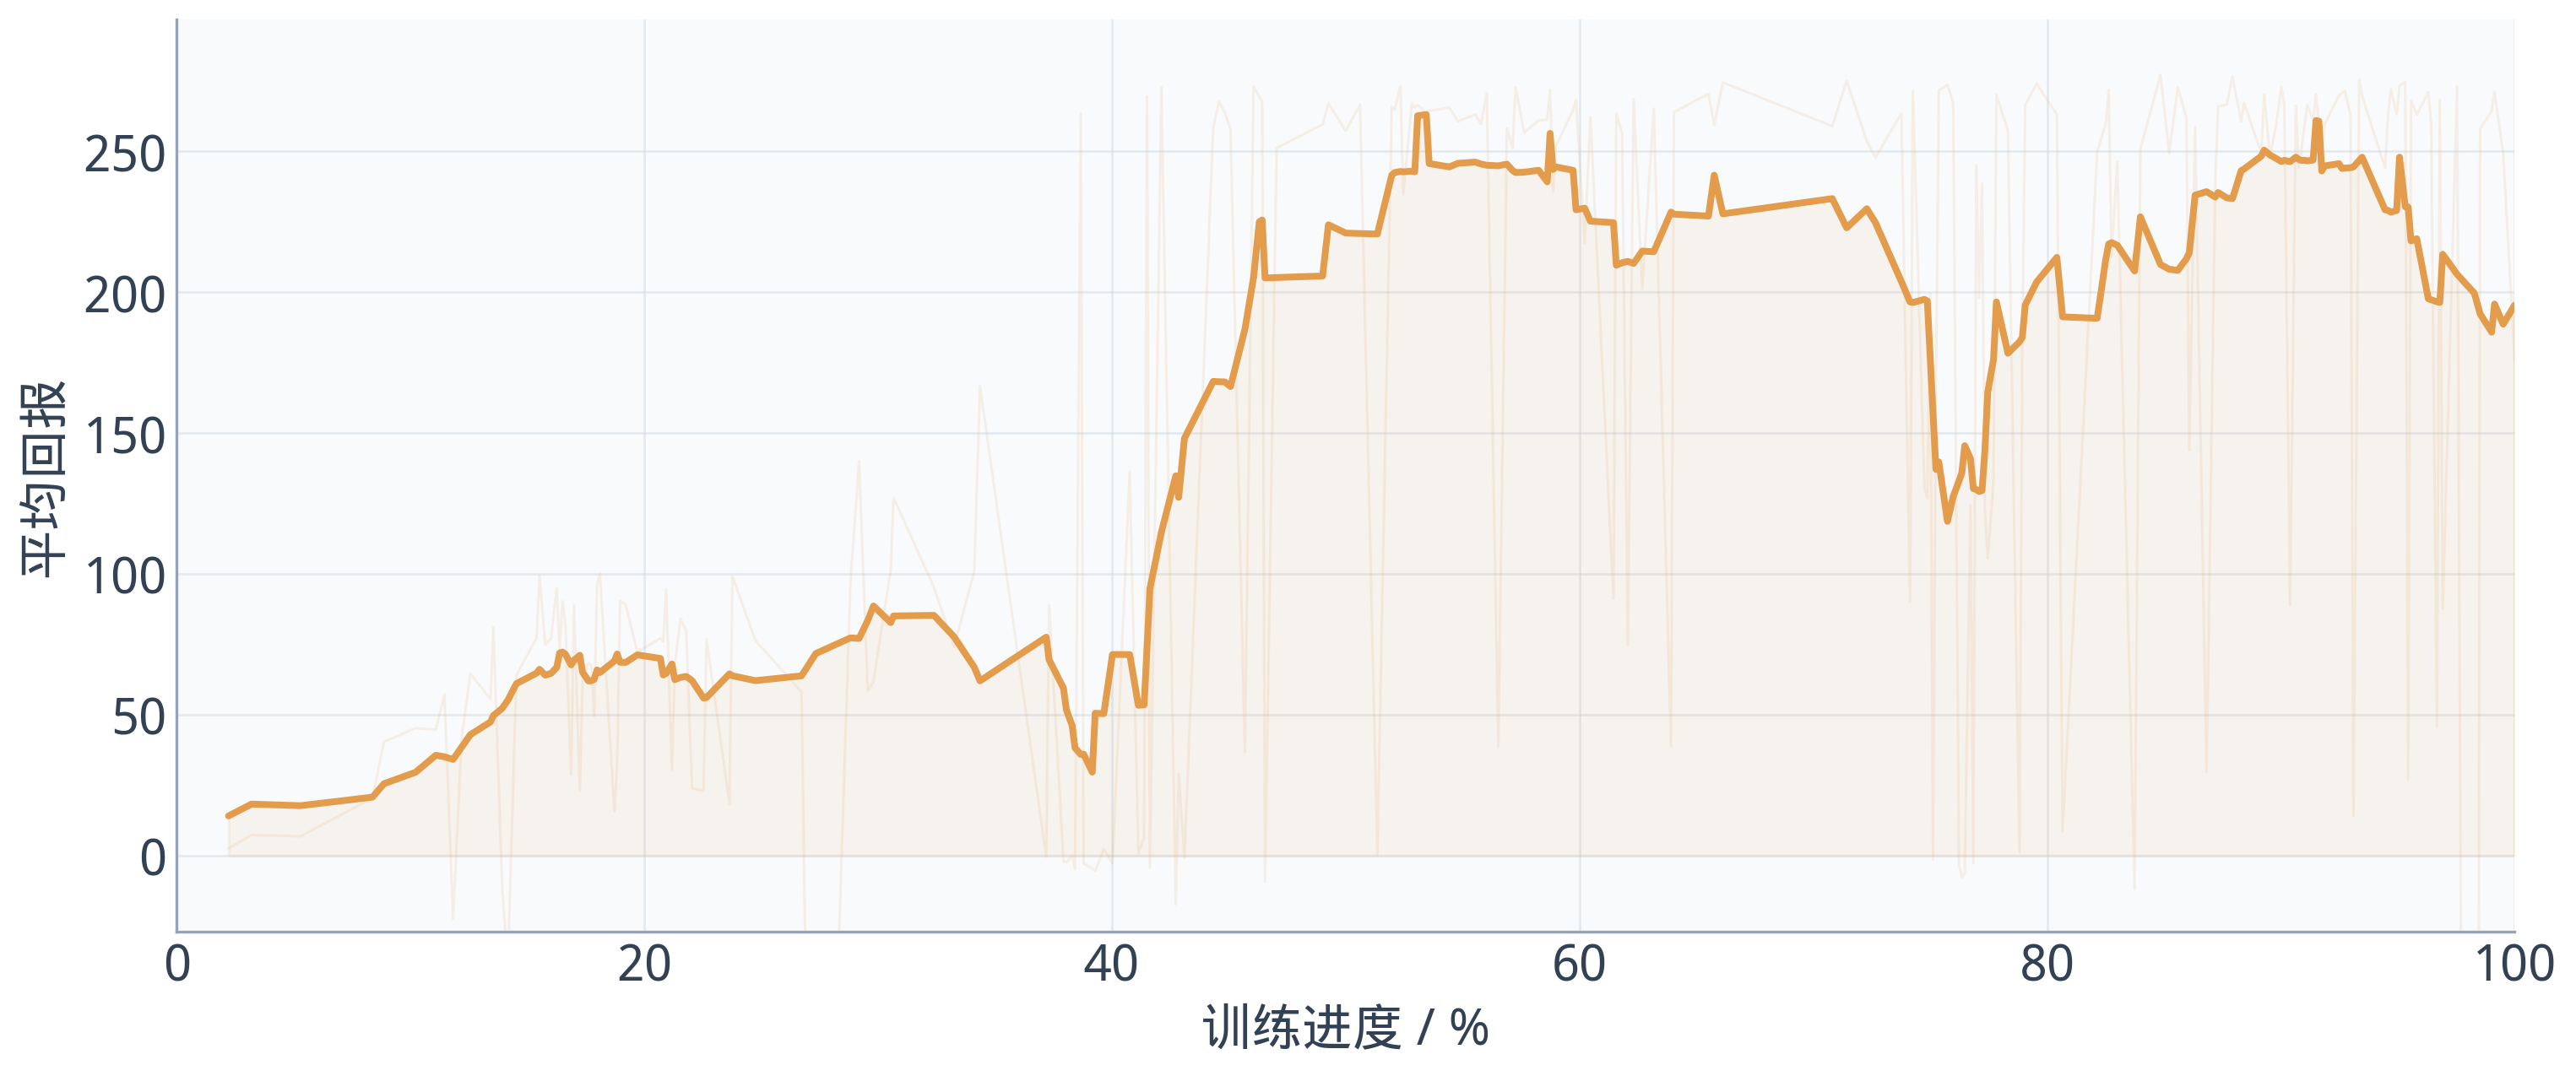
\includegraphics[width=1.22\textwidth,height=0.33\textheight,keepaspectratio]{assets/figures/rotation/stage2_base_reward_curve.png}
        \end{column}
    \end{columns}

    \vspace{0.45em}
    \begin{columns}[T,onlytextwidth]
        \begin{column}{0.49\textwidth}
            \centering
            \textbf{\textcolor{maincolor}{Teacher Playback}}\\[0.15em]
            \href{run:assets/videos/rotation/sim_teacher_success.mp4}{%
                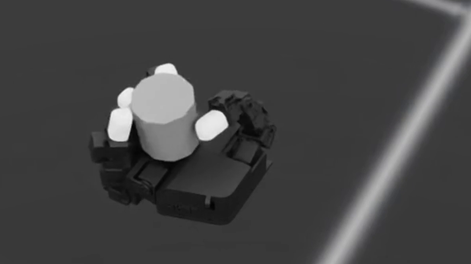
\includegraphics[width=1.14\textwidth,height=0.29\textheight,keepaspectratio]{assets/figures/rotation/teacher_success_preview_zoom.png}}

            \scriptsize privileged policy learns stable axial spin
        \end{column}
        \begin{column}{0.49\textwidth}
            \centering
            \textbf{\textcolor{maincolor}{Deploy-Base Playback}}\\[0.15em]
            \href{run:assets/videos/rotation/sim_deploy_base_success.mp4}{%
                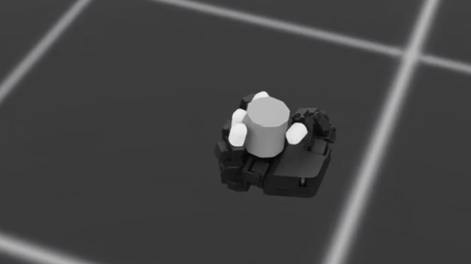
\includegraphics[width=1.14\textwidth,height=0.29\textheight,keepaspectratio]{assets/figures/rotation/deploy_base_success_preview_zoom.png}}

            \scriptsize proprioception-only policy can execute the skill
        \end{column}
    \end{columns}

\end{frame}

\begin{frame}{High-CoM OOD: Failure and Recovery}
    \footnotesize
    \vspace{0.15em}
    \begin{columns}[T,onlytextwidth]
        \begin{column}{0.49\textwidth}
            \centering
            \textbf{\textcolor{maincolor}{Deploy-Base Failure}}\\[0.15em]
            \href{run:assets/videos/rotation/sim_deploy_base_high_com_failure.mp4}{%
                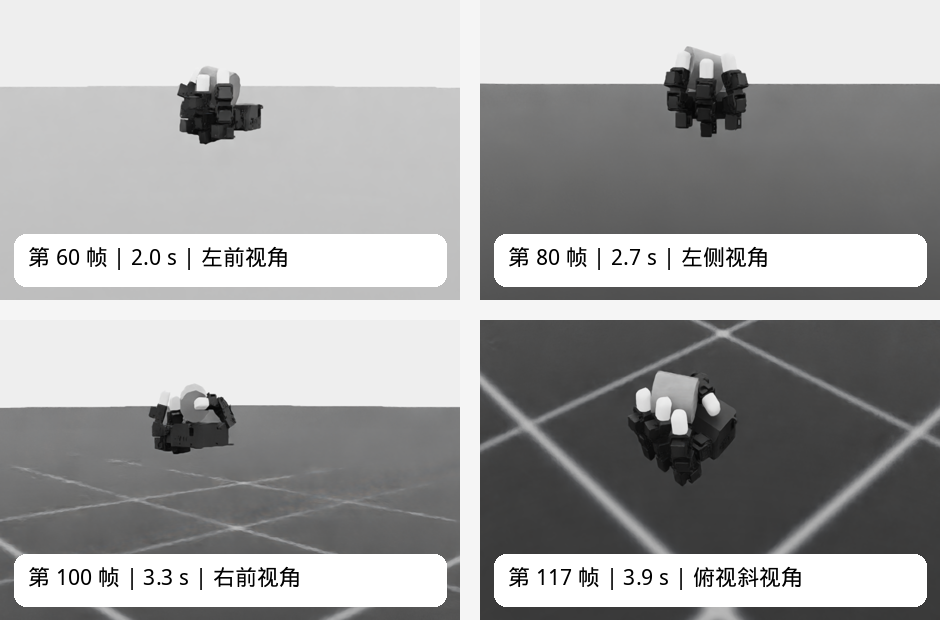
\includegraphics[width=1.12\textwidth,height=0.42\textheight,keepaspectratio]{assets/figures/rotation/base_high_com_failure_keyframes.png}}

            \scriptsize high CoM: contact drifts out
        \end{column}
        \begin{column}{0.49\textwidth}
            \centering
            \textbf{\textcolor{maincolor}{Deploy-Refined Recovery}}\\[0.15em]
            \href{run:assets/videos/rotation/sim_deploy_refined_high_com_success.mp4}{%
                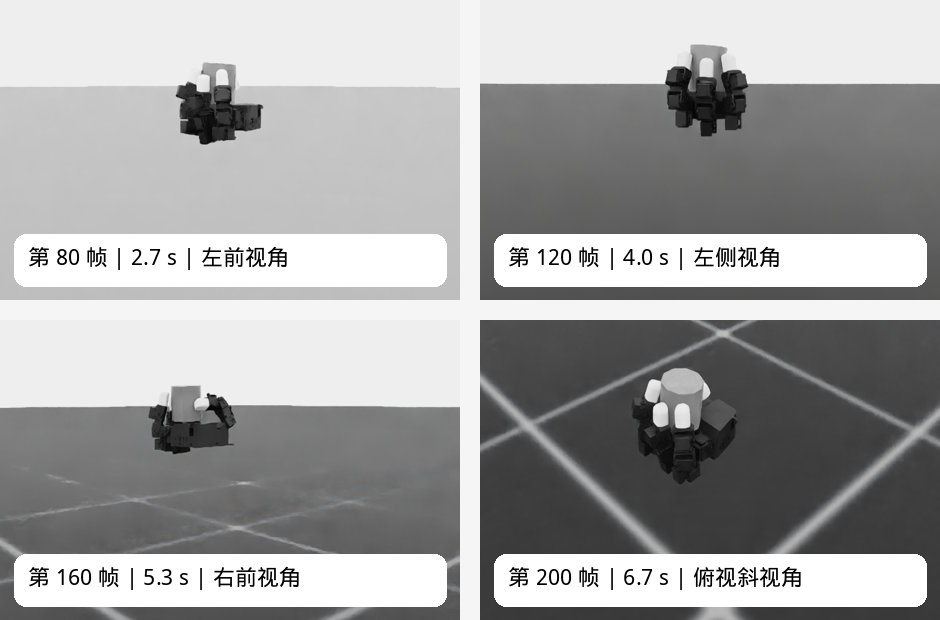
\includegraphics[width=1.12\textwidth,height=0.42\textheight,keepaspectratio]{assets/figures/rotation/refined_high_com_keyframes.png}}

            \scriptsize refined Stage 2 keeps contact
        \end{column}
    \end{columns}

    \vspace{0.35em}
    \centering
    \scriptsize
    Base training solved nominal rotation, but high CoM shifts the contact patch and exposes a deployment-side stability gap.

    \vspace{0.25em}
    \begin{columns}[T,onlytextwidth]
        \begin{column}{0.48\textwidth}
            \textbf{\textcolor{maincolor}{Observed Risk}}
            \[
                |c|>0.01\,\mathrm{m}
                \Rightarrow
                \text{OOD contact drift}
            \]
        \end{column}
        \begin{column}{0.48\textwidth}
            \textbf{\textcolor{maincolor}{Refinement}}
            \[
                L_{stage2}=L_{lat}+\lambda_{act}L_{act},
                \quad
                |c|\le0.015\,\mathrm{m}
            \]
        \end{column}
    \end{columns}
\end{frame}

\begin{frame}{Simulation Results: ID and OOD Evaluation}
    \footnotesize
    \vspace{0.55em}
    \textbf{\textcolor{maincolor}{ID Evaluation}}

    \vspace{0.15em}
    \resizebox{\textwidth}{!}{%
            \begin{tabular}{lcccccc}
                \hline
                Policy & Success$\uparrow$ & Survival$\uparrow$ & Turns$\uparrow$ & Spin$\uparrow$ & LinVel$\downarrow$ cm/s & Torque$\downarrow$ \\
                \hline
                Teacher & \textbf{1.0000} & \textbf{0.9983} & 3.6950 & 1.1628 & \textbf{3.4478} & 2.3407 \\
                Deploy-Base & 0.9922 & 0.9966 & 3.6309 & 1.1444 & 3.5378 & 2.3575 \\
                Deploy-Refined & \textbf{1.0000} & \textbf{0.9983} & \textbf{3.7081} & \textbf{1.1669} & 3.6543 & \textbf{2.3373} \\
                \hline
            \end{tabular}
    }

    \vspace{0.55em}
    \textbf{\textcolor{maincolor}{OOD Evaluation}}

    \vspace{0.15em}
    \resizebox{\textwidth}{!}{%
            \begin{tabular}{lcccccc}
                \hline
                Policy & Success$\uparrow$ & Survival$\uparrow$ & Turns$\uparrow$ & Spin$\uparrow$ & LinVel$\downarrow$ cm/s & Torque$\downarrow$ \\
                \hline
                Teacher & \textbf{0.9766} & \textbf{0.9913} & \textbf{3.4684} & \textbf{1.0956} & \textbf{3.9620} & 2.4103 \\
                Deploy-Base & 0.8750 & 0.9492 & 3.0422 & 0.9803 & 4.4935 & 2.4433 \\
                Deploy-Refined & 0.9141 & 0.9758 & 3.2558 & 1.0420 & 4.2818 & \textbf{2.4087} \\
                \hline
            \end{tabular}
    }

    \vspace{0.35em}
    \centering
    \scriptsize Deploy-Refined improves OOD success, survival, net turns, spin, linear stability, and torque cost relative to Deploy-Base.
\end{frame}

\begin{frame}{Ablations I: Deployable Skill Prior}
    \scriptsize
    \vspace{0.9em}
    \textbf{\textcolor{maincolor}{Privileged Information}}

    \vspace{0.1em}
    \resizebox{\textwidth}{!}{%
    \begin{tabular}{lcccc}
        \hline
        Setting & ID success$\uparrow$ & OOD success$\uparrow$ & OOD turns$\uparrow$ & OOD spin$\uparrow$ \\
        \hline
        Full privileged information & \textbf{0.9922} & \textbf{0.8750} & \textbf{3.0422} & \textbf{0.9803} \\
        no object position & 0.9453 & 0.6172 & 2.3078 & 0.9231 \\
        no mass / friction & 0.9375 & 0.7344 & 2.6264 & 0.9073 \\
        no CoM offset & 0.0000 & 0.0000 & 0.4247 & 0.5707 \\
        \hline
    \end{tabular}
    }

    \vspace{0.55em}
    \textbf{\textcolor{maincolor}{Representation and Temporal Interface}}

    \vspace{0.1em}
    \resizebox{\textwidth}{!}{%
    \begin{tabular}{llcccc}
        \hline
        Slice & Setting & ID success$\uparrow$ & OOD success$\uparrow$ & OOD spin$\uparrow$ & Alignment$\downarrow$ \\
        \hline
        representation & $9$D $\rightarrow$ $8$D skill prior & \textbf{0.9922} & \textbf{0.8750} & 0.9803 & -- \\
        representation & direct $9$D privilege & 0.7734 & 0.5391 & 0.4005 & -- \\
        history length & $25$ frames & \textbf{1.0000} & \textbf{0.9219} & 1.0178 & -- \\
        history length & $30$ frames & 0.9922 & 0.8906 & \textbf{1.0500} & -- \\
        encoder & Flatten-MLP & 0.9688 & 0.7969 & 0.9036 & 0.4597 \\
        encoder & 1D-CNN & 0.9922 & 0.8906 & \textbf{1.0500} & \textbf{0.3018} \\
        encoder & GRU & \textbf{1.0000} & 0.9141 & 1.0176 & 0.3147 \\
        \hline
    \end{tabular}
    }

\end{frame}

\begin{frame}{Ablations II: Why Deploy-Refined Works}
    \tiny
    \vspace{0.25em}
    \textbf{\textcolor{maincolor}{Refinement Components under OOD}}

    \vspace{0.1em}
    \resizebox{\textwidth}{!}{%
    \begin{tabular}{lccccc}
        \hline
        Stage 2 setting & Success$\uparrow$ & Survival$\uparrow$ & Turns$\uparrow$ & Spin$\uparrow$ & Action gap$\downarrow$ \\
        \hline
        Deploy-Base & 0.8750 & 0.9492 & 3.0422 & 0.9803 & -- \\
        CoM only & 0.8750 & 0.9469 & 3.0312 & 0.9847 & 0.3929 \\
        Action only & 0.8906 & 0.9640 & 3.2001 & 1.0314 & 0.3635 \\
        CoM + action & \textbf{0.9141} & \textbf{0.9758} & \textbf{3.2558} & \textbf{1.0420} & \textbf{0.3053} \\
        \hline
    \end{tabular}
    }

    \vspace{0.55em}
    \textbf{\textcolor{maincolor}{Action Consistency Weight}}

    \vspace{0.1em}
    \resizebox{\textwidth}{!}{%
    \begin{tabular}{lcccccc}
        \hline
        $\lambda_{act}$ & ID S$\uparrow$ & OOD S$\uparrow$ & Survival$\uparrow$ & Turns$\uparrow$ & Spin$\uparrow$ & Action gap$\downarrow$ \\
        \hline
        $0$ & 0.9766 & 0.8750 & 0.9469 & 3.0312 & 0.9847 & 0.3929 \\
        $0.25$ & \textbf{1.0000} & 0.8828 & 0.9551 & 3.1595 & 1.0099 & 0.4317 \\
        $0.5$ & 0.9922 & 0.8906 & 0.9417 & 3.1117 & 1.0092 & 0.4594 \\
        $1.0$ & \textbf{1.0000} & \textbf{0.9141} & \textbf{0.9758} & \textbf{3.2558} & \textbf{1.0420} & \textbf{0.3053} \\
        $2.0$ & \textbf{1.0000} & 0.8672 & 0.9483 & 3.0868 & 1.0049 & 0.3466 \\
        \hline
    \end{tabular}
    }

    \vspace{0.35em}
    \centering
    \scriptsize
    Action consistency gives the main gain; wider CoM provides the high-risk samples needed for the final combined policy.
\end{frame}

\begin{frame}{Real Hardware: Transfer and Boundary}
    \footnotesize
    \vspace{0.55em}
    \begin{columns}[T,onlytextwidth]
        \begin{column}{0.24\textwidth}
            \centering
            \textbf{\textcolor{maincolor}{Standard}}\\[0.1em]
            \href{run:assets/videos/rotation/real_standard_cylinder_success.mp4}{%
                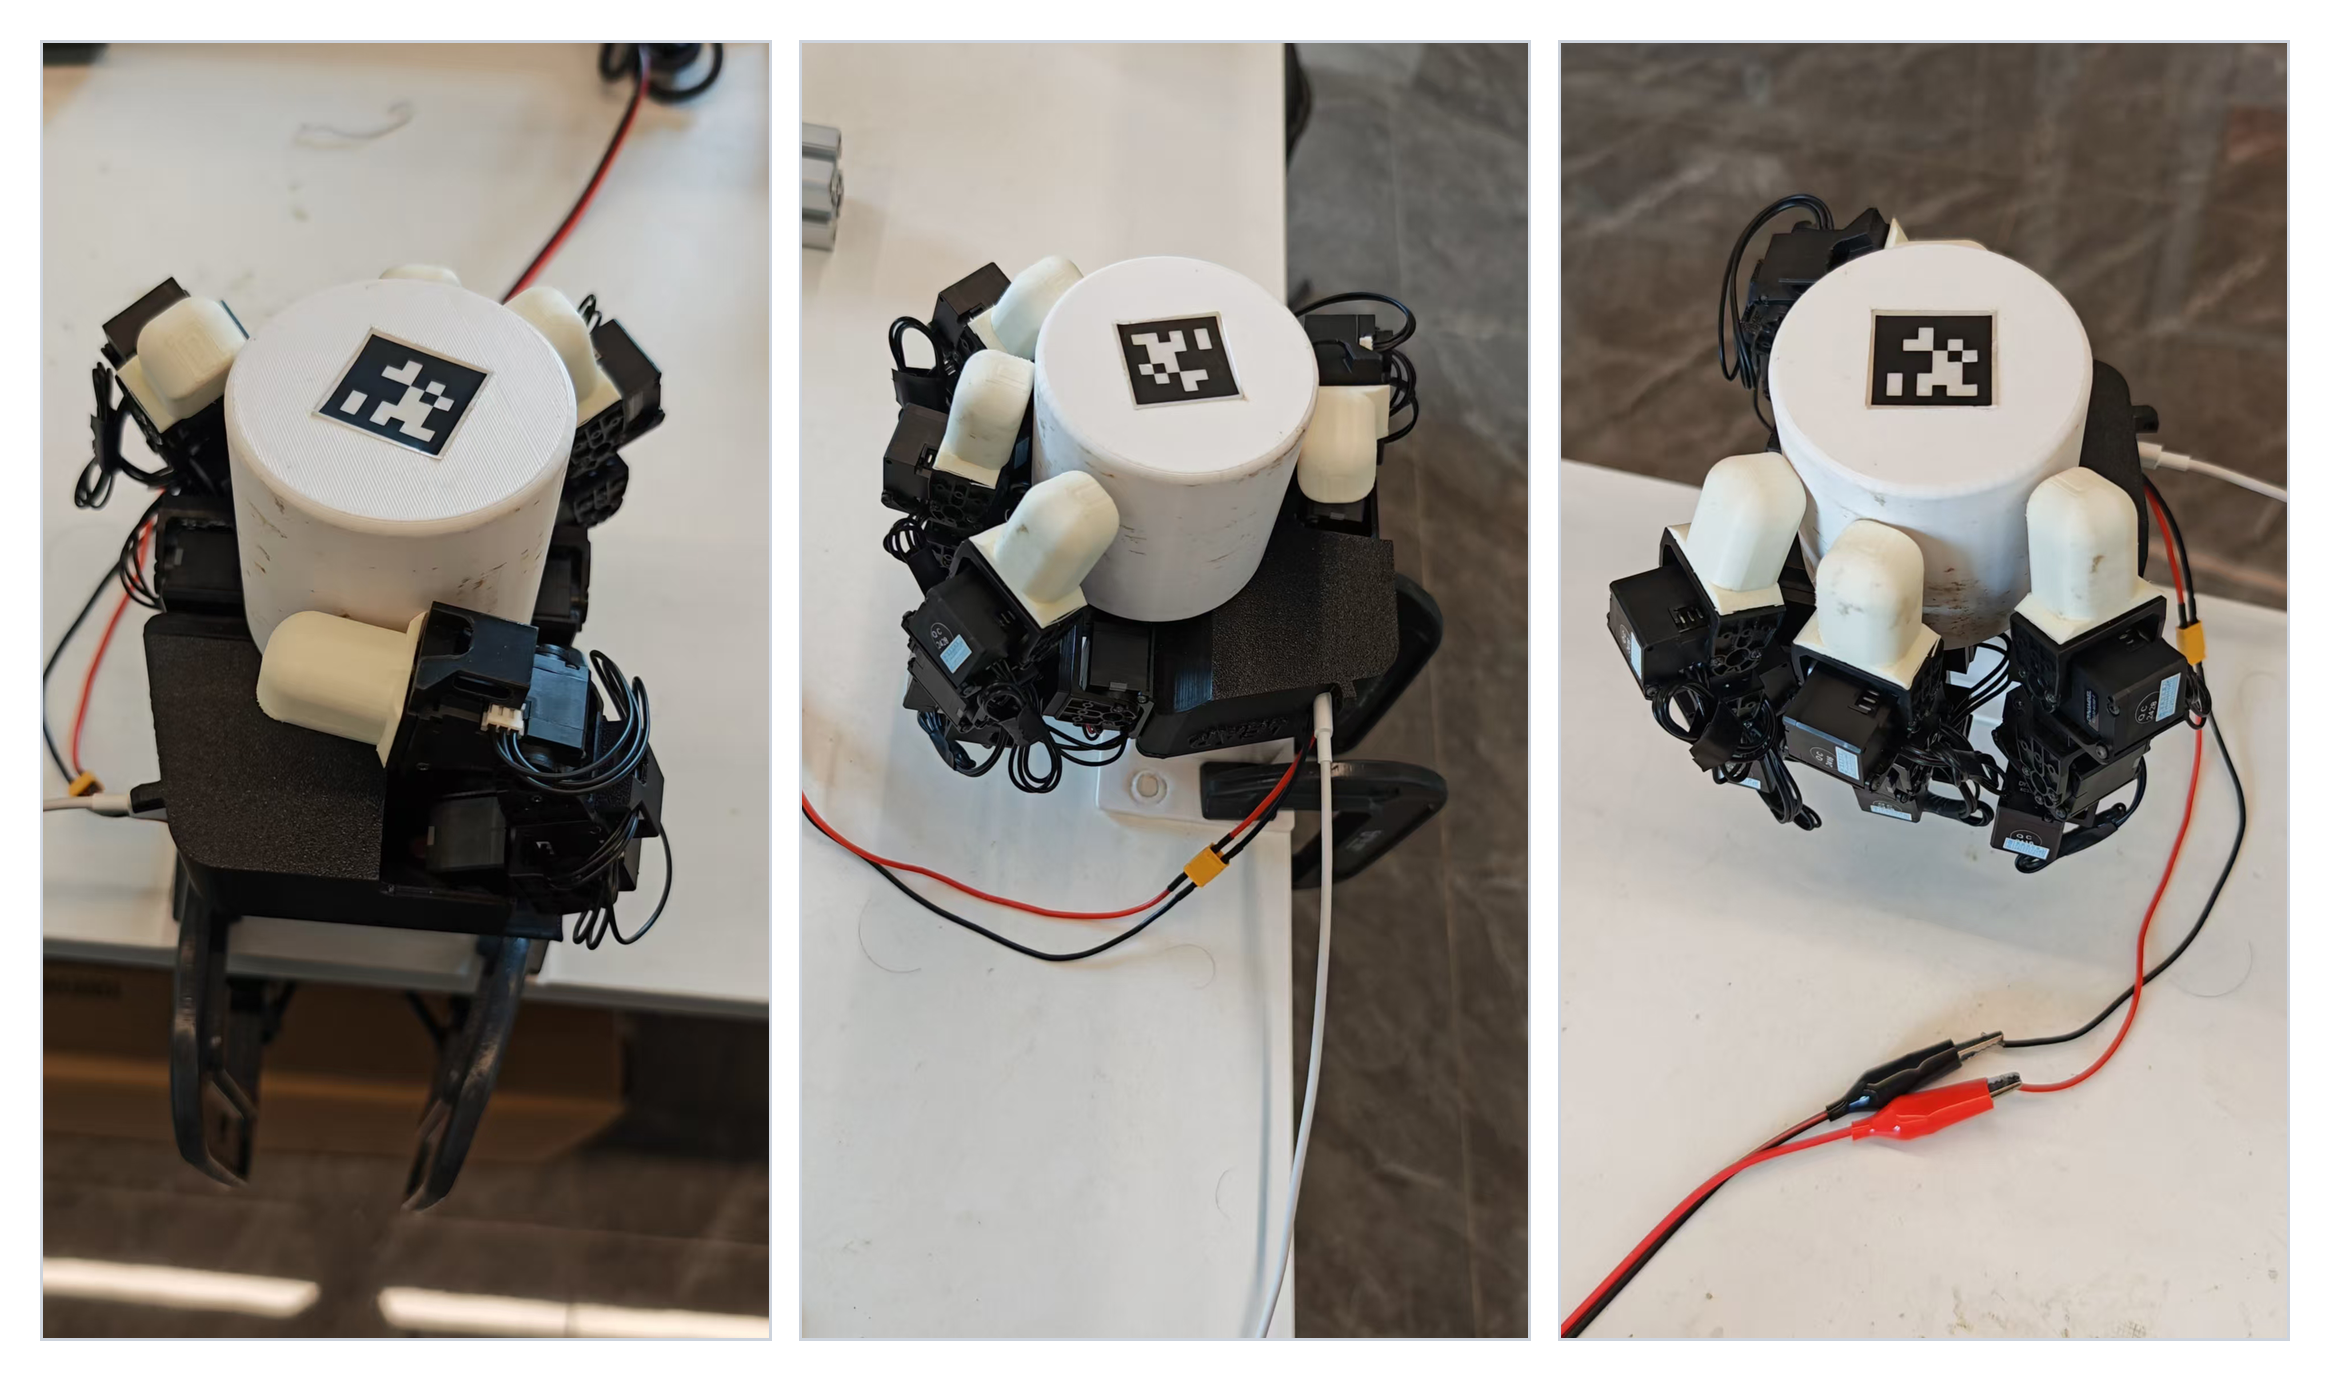
\includegraphics[width=\textwidth,height=0.26\textheight,keepaspectratio]{assets/figures/rotation/real_standard_cylinder_keyframes.png}}
        \end{column}
        \begin{column}{0.24\textwidth}
            \centering
            \textbf{\textcolor{maincolor}{Smaller}}\\[0.1em]
            \href{run:assets/videos/rotation/real_small_cylinder_success.mp4}{%
                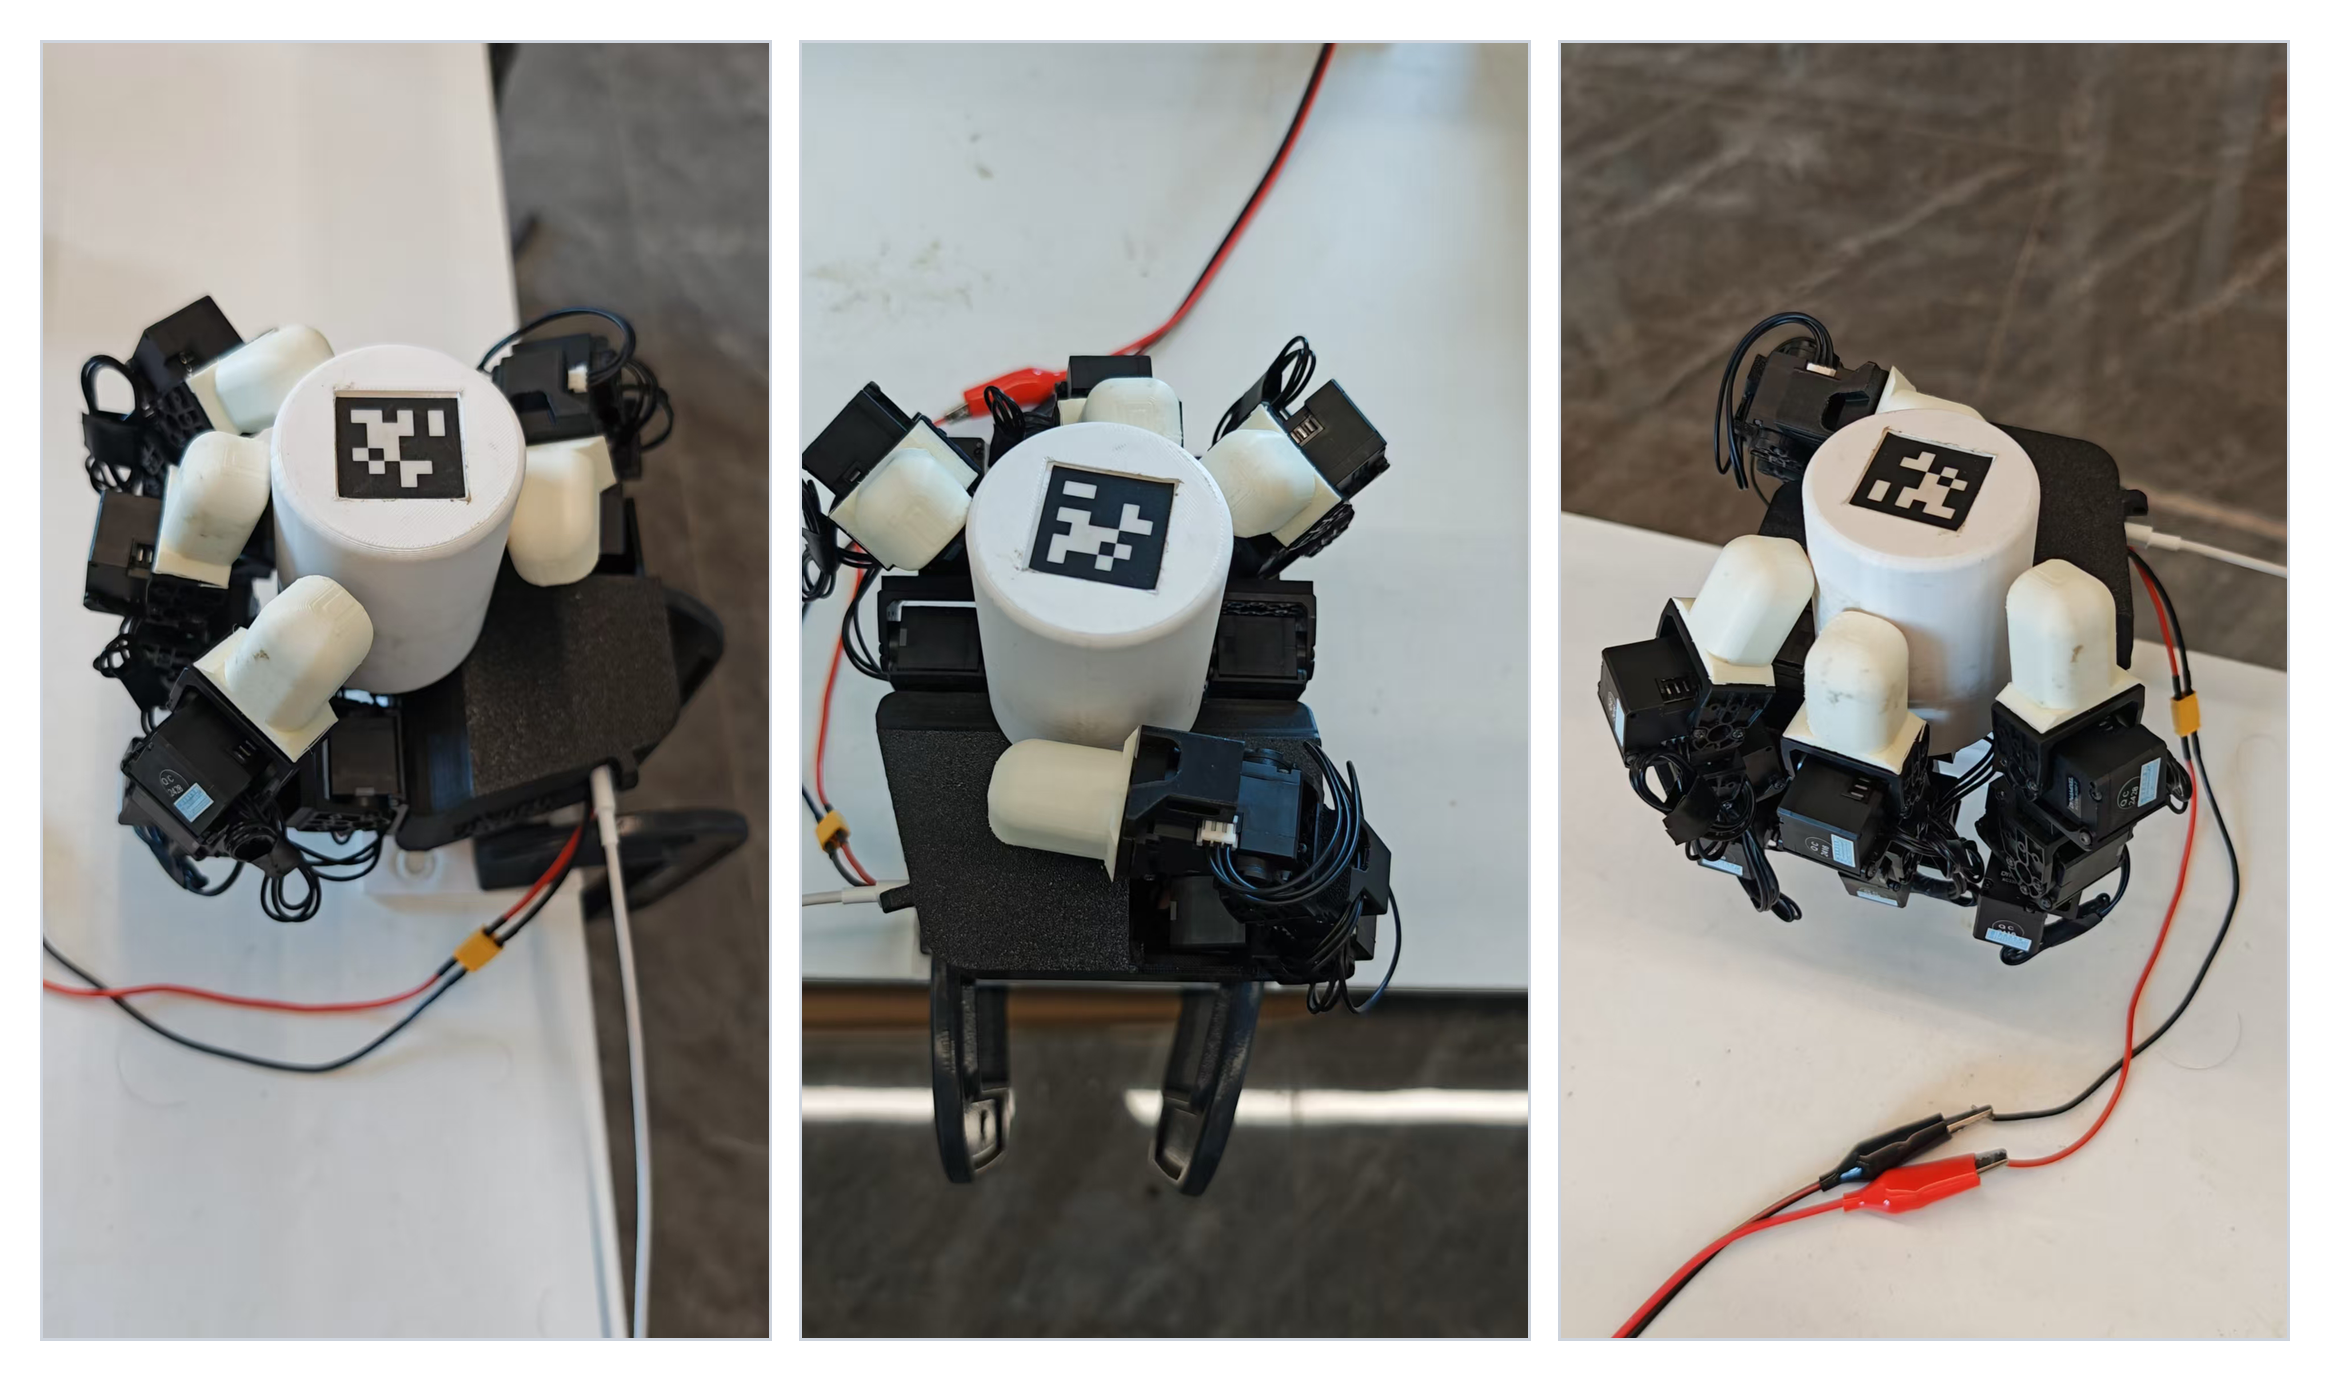
\includegraphics[width=\textwidth,height=0.26\textheight,keepaspectratio]{assets/figures/rotation/real_small_cylinder_keyframes.png}}
        \end{column}
        \begin{column}{0.24\textwidth}
            \centering
            \textbf{\textcolor{maincolor}{Slender}}\\[0.1em]
            \href{run:assets/videos/rotation/real_slender_bottle_success.mp4}{%
                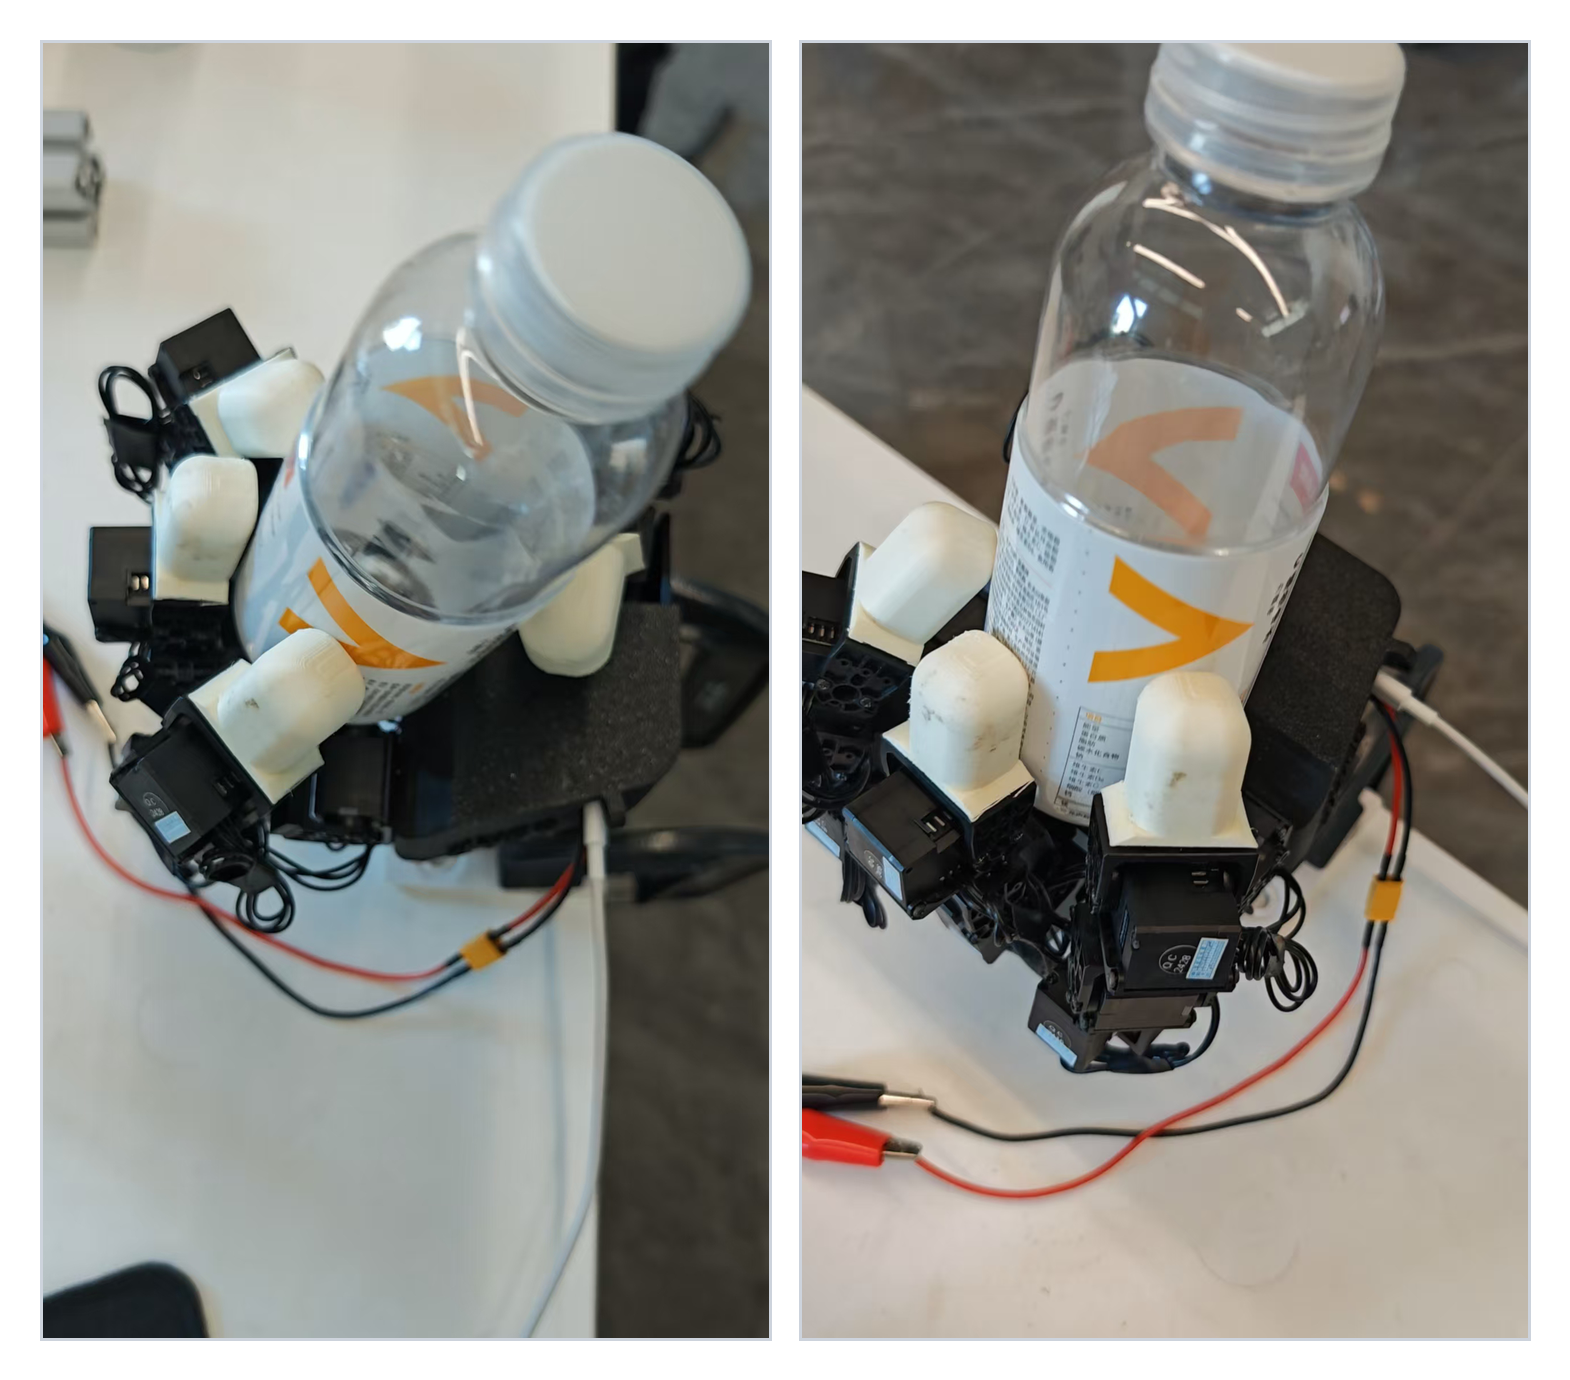
\includegraphics[width=\textwidth,height=0.26\textheight,keepaspectratio]{assets/figures/rotation/real_slender_bottle_keyframes.png}}
        \end{column}
        \begin{column}{0.24\textwidth}
            \centering
            \textbf{\textcolor{maincolor}{Ribbed}}\\[0.1em]
            \href{run:assets/videos/rotation/real_ribbed_bottle_failure.mp4}{%
                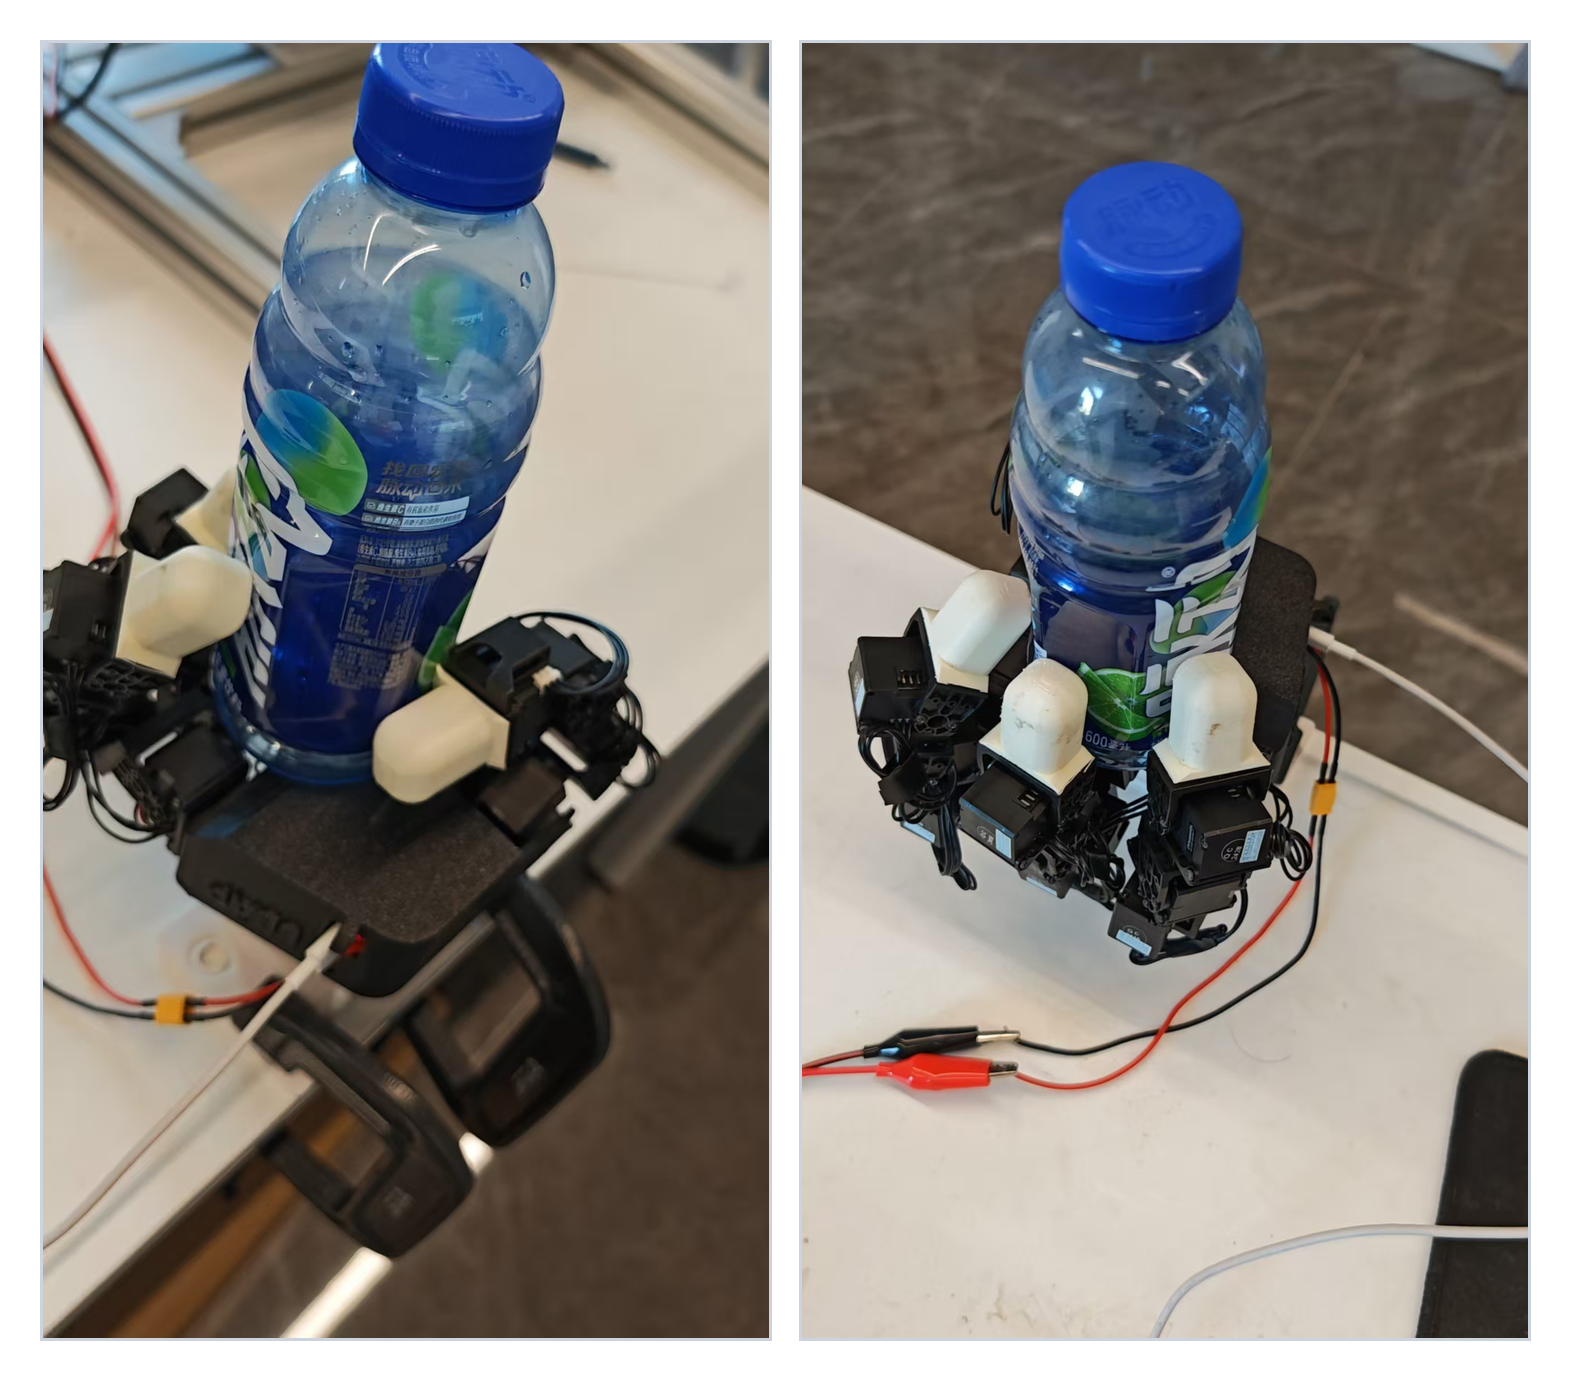
\includegraphics[width=\textwidth,height=0.26\textheight,keepaspectratio]{assets/figures/rotation/real_ribbed_bottle_keyframes.png}}
        \end{column}
    \end{columns}

    \vspace{0.35em}
    \textbf{\textcolor{maincolor}{Same Deploy-Refined Checkpoint, No Per-Object Retraining}}

    \vspace{0.15em}
    \resizebox{\textwidth}{!}{%
    \begin{tabular}{lcccc}
        \hline
        Object & Physical change & Trials$\uparrow$ & Est. turns$\uparrow$ & Failure mode \\
        \hline
        standard cylinder & training-like cylinder & \textbf{10/10} & $\sim0.5$ & none \\
        smaller cylinder & smaller radius / lower mass & \textbf{10/10} & \textbf{$\sim1.0$} & none \\
        slender bottle & near-cylinder, high aspect ratio & 8/10 & \textbf{$\sim1.0$} & tilt / fall \\
        ribbed bottle & non-round local edges & 0/10 & -- & edge jamming \\
        \hline
    \end{tabular}
    }

    \vspace{0.25em}
    \centering
    \scriptsize Boundary: current policy transfers to cylinders and near-cylinders, but not ribbed non-round contact geometry.
\end{frame}

\begin{frame}{Thesis Takeaways}
    \small
    \vspace{0.7em}
    \begin{columns}[T,onlytextwidth]
        \begin{column}{0.48\textwidth}
            \textbf{\textcolor{maincolor}{What Has Been Established}}
            \begin{itemize}
                \item A deployable LEAP Hand cylinder-rotation task.
                \item A two-stage skill-prior adaptation pipeline.
                \item ID/OOD simulation evaluation and ablations.
                \item Real hardware demos and failure boundary.
            \end{itemize}
        \end{column}
        \begin{column}{0.48\textwidth}
            \textbf{\textcolor{maincolor}{Open Problems}}
            \begin{itemize}
                \item Real rotation speed is much lower than simulation.
                \item Real object rotation is manually estimated.
                \item Non-round local geometry still breaks contact progression.
                \item Broader object generalization needs better sensing or richer training coverage.
            \end{itemize}
        \end{column}
    \end{columns}

    \vspace{0.5em}
    \centering
    \textcolor{maincolor}{Current claim: cylinder and near-cylinder rotation, not arbitrary-object rotation.}
\end{frame}

\section{Future Work}

\begin{frame}{From Joint-Space Policy to Hand Geometry}
    \small
    \vspace{0.65em}
    \begin{columns}[T,onlytextwidth]
        \begin{column}{0.47\textwidth}
            \textbf{\textcolor{maincolor}{Current Policy}}
            \begin{itemize}
                \item 16D relative joint targets.
                \item Proprioception-only deployment.
                \item Cylinder and near-cylinder rotation works.
            \end{itemize}
        \end{column}
        \begin{column}{0.47\textwidth}
            \textbf{\textcolor{maincolor}{Observed Boundary}}
            \begin{itemize}
                \item Ribbed or non-round geometry causes contact jamming.
                \item Hand shape and contact geometry are implicit.
                \item Generalization depends heavily on training coverage.
            \end{itemize}
        \end{column}
    \end{columns}

    \vspace{0.85em}
    \centering
    \fbox{%
        \begin{minipage}{0.88\textwidth}
            \centering
            \textbf{\textcolor{maincolor}{Research Problem}}\\[0.25em]
            Can contact-relevant hand keypoints reduce learning complexity while preserving dexterous adaptability?

            \vspace{0.35em}
            \scriptsize
            \textcolor{maincolor}{Structure:} contact-envelope action prior
            \quad
            \textcolor{maincolor}{Freedom:} learned residual correction
        \end{minipage}
    }
\end{frame}

\begin{frame}{Affine Transformation on Hand Keypoints}
    \small
    \vspace{0.55em}
    \begin{columns}[T,onlytextwidth]
        \begin{column}{0.48\textwidth}
            \textbf{\textcolor{maincolor}{Key Representation}}
            \[
                P_i^\ast = A P_i^0 + b
            \]

            \vspace{0.2em}
            \begin{itemize}
                \item \(P_i^0\): nominal contact-relevant hand keypoint.
                \item \(A\): scaling, rotation, and shear.
                \item \(b\): translation.
                \item \(P_i^\ast\): target hand-shape keypoint.
            \end{itemize}

            \vspace{0.25em}
            \textcolor{maincolor}{The affine transform is applied to hand keypoints, not directly to joint angles.}
        \end{column}
        \begin{column}{0.48\textwidth}
            \textbf{\textcolor{maincolor}{Control Pipeline}}

            \vspace{0.55em}
            \centering
            \begin{tabular}{c}
                \fbox{\parbox{0.78\linewidth}{\centering Nominal hand keypoints}} \\
                \(\downarrow\) affine transform \\
                \fbox{\parbox{0.78\linewidth}{\centering Target hand keypoints}} \\
                \(\downarrow\) IK or learned mapping \\
                \fbox{\parbox{0.78\linewidth}{\centering LEAP Hand joint targets}}
            \end{tabular}

            \vspace{0.75em}
            \scriptsize
            Candidate nodes: palm reference, finger-link surface points, fingertips, and contact proxies.
        \end{column}
    \end{columns}
\end{frame}

\begin{frame}{Initial Research Plan}
    \small
    \vspace{1.25em}
    \begin{columns}[T,onlytextwidth]
        \begin{column}{0.32\textwidth}
            \textbf{\textcolor{maincolor}{1. Define Contact Keypoints}}
            \begin{itemize}
                \item palm / in-hand reference;
                \item finger-link surface points;
                \item fingertips only if useful.
            \end{itemize}
        \end{column}
        \begin{column}{0.32\textwidth}
            \textbf{\textcolor{maincolor}{2. Build Affine Prior}}
            \begin{itemize}
                \item start from nominal grasp shapes;
                \item scale, rotate, and shear keypoints;
                \item map keypoints to joint targets.
            \end{itemize}
        \end{column}
        \begin{column}{0.32\textwidth}
            \textbf{\textcolor{maincolor}{3. Compare Interfaces}}
            \begin{itemize}
                \item direct 16D joint-space policy;
                \item affine-only policy;
                \item affine plus residual policy.
            \end{itemize}
        \end{column}
    \end{columns}

    \vspace{0.8em}
    \textbf{\textcolor{maincolor}{Evaluation}}
    \begin{itemize}
        \item object size variation;
        \item object orientation variation;
        \item near-cylinder versus non-round geometry.
    \end{itemize}

    \vspace{0.35em}
    \centering
    \textcolor{maincolor}{Goal: keep the existing sim-to-real pipeline, but improve geometric generalization.}
\end{frame}

\QApage

\end{document}
